\documentclass[10pt]{beamer}
\usetheme{Frankfurt}
\usepackage[utf8]{inputenc}
\usepackage[spanish,es-tabla]{babel}
%\usepackage[T1]{fontenc}
\usepackage{amsmath}
\usepackage{amsfonts}
\usepackage{amssymb}
\usepackage{graphicx}
\graphicspath{{imagenes/}}
\author{Ciro Fabián Bermúdez Márquez}
\title{TRNGs para generación de secuencias muy largas}
\institute{Instituto Nacional de Astrofísica, Óptica y Electrónica} 
\date{\today} 

%-------------------------------------------------------------------------------
%                            Paquetes adicionales                              %
%-------------------------------------------------------------------------------
%-------------------------------------------------------------------------------
%                                Paquetes extras                               %
%-------------------------------------------------------------------------------
\setcounter{secnumdepth}{3}
\setcounter{tocdepth}{3} 
\usepackage{amsthm}
\theoremstyle{definition}
\newtheorem{axiom}{Axioma} %[chapter]
\renewcommand\theaxiom{\Roman{axiom}}

\theoremstyle{definition}
\newtheorem{property}{Propiedad} %[chapter]

\theoremstyle{definition}
\newtheorem{corollary}{Corolario} %[chapter]

\theoremstyle{definition}
\newtheorem{theorem}{Teorema} %[chapter]

\usepackage{lipsum}												% Texto de ejemplo \lipsum[1-30]
\decimalpoint													% Punto decimal en lugar de coma
\spanishsignitems												% Viñetas en lugar de cuadros
\raggedbottom													% Eliminar molestos warnings

\usepackage{comment}											% Comentarios largos
\usepackage{pdfpages}											% Incluir portada echa en Inkscape
\usepackage{setspace}											% Interlineado
\usepackage{makecell}											% Para tablas
\usepackage{xcolor}												% Colores en tablas
\usepackage{colortbl}
\usepackage{multirow}
\usepackage{array}												% Necesario para algunas tablas
\usepackage[inline]{enumitem}									% Personalizar itemize
\usepackage{multicol}											% Item 2 columns

\definecolor{Red}{RGB}{255,191,191}								% Colores definidos por el usuario

\usepackage[nottoc]{tocbibind}									% Bibliografia en table of contents

\usepackage[figuresright]{rotating}								% Rotar figuras con caption
\usepackage{subcaption}											% Subfiguras
%-------------------------------------------------------------------------------
%                            Comandos matematicos                              %
%-------------------------------------------------------------------------------
\usepackage{steinmetz}											% Para representar fasores
\usepackage{bm}													% Bold math  \bm command
\newcommand{\binomb}[2]{\genfrac{[}{]}{0pt}{}{#1}{#2}}
%-------------------------------------------------------------------------------
%                        Paquetes para hipervinculos                           %
%-------------------------------------------------------------------------------
\usepackage[hidelinks]{hyperref}								% Añade los bookmarks y le quita la caja roja, \url{}
\urlstyle{same}
%-------------------------------------------------------------------------------
%                           Estilos de encabezados                             %
%-------------------------------------------------------------------------------
\usepackage{fancyhdr, blindtext}								% Libreria para encabezados

\renewcommand{\chaptermark}[1]{\markboth{#1}{}}					% Capitulos y secciones en minusculas
\renewcommand{\sectionmark}[1]{\markright{#1}}

\fancypagestyle{normalstyle}{%
  \fancyhf{}													% Reinicial estilos de header y footer
	\fancyhead[LE,RO]{\thepage}
	\fancyhead[LO]{\nouppercase{\rightmark}}
	\fancyhead[RE]{\nouppercase{\leftmark}}
	\renewcommand{\headrulewidth}{0.4pt}
	\renewcommand{\footrulewidth}{0pt}
	\setlength{\headheight}{14.62pt}
}

\fancypagestyle{Resumen}{%
  \fancyhf{}													% Reinicial estilos de header y footer
	\fancyhead[LE,RO]{\thepage}
	\fancyhead[LO]{\nouppercase{Resumen}}
	\fancyhead[RE]{\nouppercase{Resumen}}
	\renewcommand{\headrulewidth}{0.4pt}
	\renewcommand{\footrulewidth}{0pt}
	\setlength{\headheight}{14.62pt}
}
%-------------------------------------------------------------------------------
%                            Libreria de codigos                               %
%-------------------------------------------------------------------------------
% Paquetes necesarios
\usepackage{listings}
\usepackage{xcolor}

% Colores para tablas
\definecolor{Gray}{RGB}{230,230,230}
\definecolor{Red}{RGB}{255,191,191}

% Colores personalizados
\definecolor{verde}{rgb}{0,0.6,0}
\definecolor{gris}{RGB}{253, 253, 253}
\definecolor{grisfuerte}{RGB}{140, 140, 140}

% Deficion de lenguajes perzonalizados

% Estilos MATLAB
\lstdefinestyle{MATLAB}{
	language=MATLAB,
	basicstyle=\linespread{1}\tiny\fontfamily{pcr}\selectfont,
	backgroundcolor=\color{gris},
	frame=single,
	frameround=tttt,
	rulecolor=\color{black},
	commentstyle=\color{verde},
	keywordstyle=\color{blue}, %magenta
	stringstyle=\color{grisfuerte},                  
	captionpos=t,                    
	breaklines=true,                       
	breakatwhitespace=false,
	showspaces=false,                
	showstringspaces=false,
	showtabs=false,
	keepspaces=true,
	columns=flexible,
	tabsize=4,   
}

\lstdefinestyle{VHDL}{
	language=VHDL,
	basicstyle=\linespread{1}\tiny\fontfamily{pcr}\selectfont,
	backgroundcolor=\color{gris},
	frame=single,
	frameround=tttt,
	rulecolor=\color{black},
	commentstyle=\color{verde},
	keywordstyle=\color{blue}, %magenta
	stringstyle=\color{grisfuerte},                  
	captionpos=t,                    
	breaklines=true,                       
	breakatwhitespace=false,
	showspaces=false,                
	showstringspaces=false,
	showtabs=false,
	keepspaces=true,
	columns=flexible,
	tabsize=4,
	upquote=true,
}


\lstdefinestyle{VHDL_TEXT}{
	language=VHDL,
	basicstyle=\linespread{1}\footnotesize\fontfamily{pcr}\selectfont,
	backgroundcolor=\color{gris},
	frame=single,
	frameround=tttt,
	rulecolor=\color{black},
	commentstyle=\color{verde},
	keywordstyle=\color{blue}, %magenta
	stringstyle=\color{grisfuerte},                  
	captionpos=t,                    
	breaklines=true,                       
	breakatwhitespace=false,
	showspaces=false,                
	showstringspaces=false,
	showtabs=false,
	keepspaces=true,
	columns=flexible,
	tabsize=4,
	upquote=true,
}


\lstdefinestyle{C}{
	language=C,
	basicstyle=\linespread{1}\tiny\fontfamily{pcr}\selectfont,
	backgroundcolor=\color{gris},
	frame=single,
	frameround=tttt,
	rulecolor=\color{black},
	commentstyle=\color{verde},
	keywordstyle=\color{blue}, %magenta
	stringstyle=\color{grisfuerte},                  
	captionpos=t,                    
	breaklines=true,                       
	breakatwhitespace=false,
	showspaces=false,                
	showstringspaces=false,
	showtabs=false,
	keepspaces=true,
	columns=flexible,
	tabsize=4,
	upquote=true,    
}

\renewcommand{\lstlistingname}{Código}% Listing -> Algorithm
\renewcommand{\lstlistlistingname}{Lista de códigos}% 

%-------------------------------------------------------------------------------
%                           Caption en negritas                                %
%-------------------------------------------------------------------------------
\usepackage[labelfont=bf]{caption}
\captionsetup{labelfont=bf}


%-------------------------------------------------------------------------------
%                           Lista de conceptos                                %
%-------------------------------------------------------------------------------
\usepackage[nonumberlist,nogroupskip,toc,style=super]{glossaries}
\setlength{\glsdescwidth}{0.7\textwidth}

\makeglossaries

\newglossaryentry{FPGA}
{
    name=FPGA, %% $\qquad\qquad\qquad\qquad$
    description={Field Programmable Logic Array}
}

\newglossaryentry{RNG}
{
    name=RNG,
    description={Random Number Generator}
}

\newglossaryentry{TRNG}
{
    name=TRNG,
    description={True Random Number Generator}
}

\newglossaryentry{TERO}
{
    name=TERO,
    description={Transient Effect Ring Oscillator}
}

\newglossaryentry{ERO-TRNG}
{
    name=ERO-TRNG,
    description={Elementary ring oscillator based TRNG}
}

\newglossaryentry{COSO-TRNG}
{
    name=COSO-TRNG,
    description={Coherent sampling ring oscillator based TRNG}
}

\newglossaryentry{MURO-TRNG}
{
    name=MURO-TRNG,
    description={Multi-ring oscillator based TRNG}
}


\newglossaryentry{TERO-TRNG}
{
    name=TERO-TRNG,
    description={Transient effect ring oscillator based TRNG}
}

\newglossaryentry{PLL-TRNG}
{
    name=PLL-TRNG,
    description={Phase-locked loop based TRNG}
}


\newglossaryentry{STR-TRNG}
{
    name=STR-TRNG,
    description={Self-timed ring based TRNG}
}




\begin{document}

% Slide
\begin{frame}[plain]
    \fontfamily{cmr}\selectfont
	\begin{center}
		\textbf{Instituto Nacional de Astrofísica, Óptica y Electrónica (INAOE)}
	\end{center}
	
	\begin{figure}[hbtp]
		\centering
		
\includegraphics[width = 2cm]{Inaoe} 
	\end{figure}
	
	\begin{center}
		Maestría en Ciencias en Electrónica
	\end{center}
					
	\begin{center}
		\begin{Large}
		\textcolor{blue}{TRNGs para generación de secuencias muy largas}
		\end{Large}
	\end{center}
	
	\begin{center}
		\textbf{Autor:} Ciro Fabián Bermúdez Márquez
	\end{center}
	
	\begin{flushleft}
		\textbf{Asesor:} Dr. Esteban Tlelo Cuautle (INAOE)\\
	    \textbf{Coasesor:} Dr. Cuauhtemoc Mancillas López (CINVESTAV IPN)
	\end{flushleft}
	
	\begin{flushright}
	    \today
	\end{flushright}
\end{frame}

% Slide
\begin{frame}
    \tableofcontents
\end{frame}

\section{Introducción}


% Slide
\begin{frame}
    \frametitle{Introducción}
    \begin{block}{Números aleatorios}
        \justifying
        Los números aleatorios son valores numéricos que se generan de manera impredecible o aparentemente sin ningún patrón discernible. Tienen dos requisitos básicos.
        \begin{itemize}
            \item Buenas propiedades estadísticas. 
            \begin{itemize}
                 \item Distribución de probabilidad uniforme.
                 \item Pasar pruebas estadísticas.
            \end{itemize}
            \item Imprevisibilidad del número aleatorio.
            \begin{itemize}
                \item No debe haber correlaciones o dependencias entre ellos.
            \end{itemize}
        \end{itemize}
	\end{block}
\end{frame}


% Slide
\begin{frame}
    \frametitle{Introducción}
    \begin{block}{Aplicaciones}
        \justifying
        \begin{figure}[!h]
				\begin{minipage}[t]{0.48\textwidth}
					\begin{itemize}
								\justifying
								\item[•] Simuladores.
                                 \item[•] Muestreo estadístico.
                                 \item[•] Prueba de algoritmos.
                                 \item[•] Análisis numérico.
					\end{itemize}
				\end{minipage} \hfill \begin{minipage}[t]{0.48\textwidth}
					\begin{itemize}
								\justifying
								\item[•] Estética en imágenes.
                                 \item[•] Teoría de juegos.
                                 \item[•] Criptografía.
					\end{itemize}
				\end{minipage}
		\end{figure}
	\end{block}
	
     \begin{block}{Aplicaciones criptográficas}
        \justifying
        \begin{figure}[!h]
				\begin{minipage}[t]{0.48\textwidth}
					\begin{itemize}
								\justifying
								\item[•] Claves criptográficas.
                                 \item[•] Números de un solo uso.
                                 \item[•] Valores de relleno.
                                 
					\end{itemize}
				\end{minipage} \hfill \begin{minipage}[t]{0.48\textwidth}
					\begin{itemize}
								\justifying
								\item[•] Vectores de inicialización.
								\item[•] Desafíos.
								\item[•] Máscaras aleatorias.
					\end{itemize}
				\end{minipage}
		\end{figure}
	\end{block}	
	
\end{frame}


% Slide
\begin{frame}
    \frametitle{Introducción}
    \begin{block}{Caos}
        \justifying
        Es un comportamiento aperiódico, aparentemente impredecible, en sistemas deterministas los cuales presentan extrema sensibilidad a las condiciones iniciales, el más mínimo cambio en la condición inicial produce un resultado muy diferente \cite{Strogatz1994}.
        \vspace{0.5cm}
        
        Según \cite{Sprott2003} los sistemas caóticos tienen las siguientes características:

        \begin{itemize}
            \item[•] Son aperiódicos. % es decir nunca se repiten.
            \item[•] Presentan una dependencia sensible de las condiciones iniciales. % (y, por tanto, son imprevisibles a largo plazo).
            \item[•] Se rigen por uno o varios parámetros de control. %  una pequeña modificación de los cuales puede hacer aparecer o desaparecer el caos.
            \item[•] Sus ecuaciones son no lineales.
        \end{itemize}
	\end{block}
\end{frame}


% Slide
\section{Objetivos}
\begin{frame}
    \frametitle{Objetivos}
    \begin{block}{Objetivo general}
        \justifying
        Diseñar e implementar en FPGA un TRNG híbrido para la generación de secuencias muy largas.
	\end{block}

    \begin{block}{Objetivo específicos}
        \justifying
        \begin{itemize}
            \item[•] Investigar el estado del arte de diferentes generadores de números aleatorios.
            \item[•] Estudiar los diferentes tipos de generadores de números aleatorios y analizar sus características principales.
            \item[•] Estudiar la teoría de los mapas caóticos y su utilidad en generadores de números aleatorios.
            \item[•] Diseñar un generador de números aleatorios híbrido utilizando un TRNG como generador de semillas y un mapa caótico para realizar un postprocesamiento que mejore sus características estadísticas y comprobar estas utilizando las pruebas NIST.
            \item[•] Implementar el TRNG híbrido en una FPGA.
        \end{itemize}
	\end{block}

\end{frame}


\section{Generadores de números aleatorios (RNGs)}

% Slide 
\begin{frame}
    \frametitle{Generadores de números aleatorios (RNGs)}
    \begin{block}{Agencias de estandarización}
        \justifying
        Agencias de estandarización como:
        \begin{itemize}
            \item NIST (National Institute of Standards and Technology) \cite{Turan2018} en Estados Unidos.
            \item BSI (Federal Office for Information Security) \cite{AIS2011} en Alemania.
        \end{itemize}
        han creado una serie documentaciones, recomendaciones y pruebas estadísticas para evaluar los generadores de números aleatorios.
	\end{block}

\end{frame}


% Slide 
\begin{frame}
    \frametitle{Generadores de números aleatorios (RNGs)}
    \begin{block}{Estructura de los TRNG}
        \justifying
        Diagrama de bloques de un TRNG según las especificaciones de AIS-20/31 y NIST 800-90B.
	\end{block}
	
	\begin{figure}[hbtp]
	    \centering
	    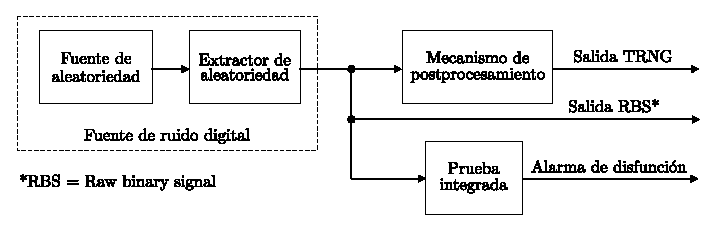
\includegraphics[width=0.8\textwidth]{A0_TRNG_estructura}
	    \caption{Estructura general de un TRNG \cite{Badrignans2011}.}
        \label{fig:A1_TRNG_estructura}
    \end{figure}
\end{frame}

% Slide 
\begin{frame}
    \frametitle{Generadores de números aleatorios (RNGs)}
    \begin{block}{Clasificación de los TRNG}
        \justifying
        Random Number Generators (RNG)
        \begin{itemize}
            \item True Random Number Generators (TRNG).
            \begin{itemize}
                \item Físicos (PTRNG).
                \item No físicos (NPTRNG).
            \end{itemize}
            \item Deterministic Random Number Generators (DRNG).
            \item Hibrid Random Number Generators (HRNG).
            \begin{itemize}
                \item HTRNG.
                \item HDRNG.
            \end{itemize}
        \end{itemize}
	\end{block}
\end{frame}


% Slide 
\begin{frame}
    \frametitle{Generadores de números aleatorios (RNGs)}
    \begin{block}{Características de los generadores}
        \justifying
        Random Number Generators (RNG)
       \begin{footnotesize}
            \begin{itemize}
            \item True Random Number Generators (TRNG).
            \begin{itemize}
                \item Fenómenos aleatorios no algorítmicos (temperatura, ruido, jitter).
                \item Datos aleatorios reales (no se pueden predecir).
                \item Propiedades estadísticas peores que DRNG.
                \item Más lentos que los DRNG.
            \end{itemize}
            \item Deterministic Random Number Generators (DRNG).
            \begin{itemize}
                \item Buenas propiedades estadísticas.
                \item Algoritmo subyacente.
                \item Semillas.
                \item Altas tasas de bits de salida.
            \end{itemize}
            \item Hibrid Random Number Generators (HRNG).
            \begin{itemize}
                \item Combinan las fortalezas de los DRNG (rápidos y de buena calidad) sembrados repetidamente por un TRNG (lento pero impredecible).
            \end{itemize}
        \end{itemize}
       \end{footnotesize}
	\end{block}
\end{frame}


% Slide 
\begin{frame}
    \frametitle{Generadores de números aleatorios (RNGs)}
	\begin{figure}[hbtp]
	    \centering
	    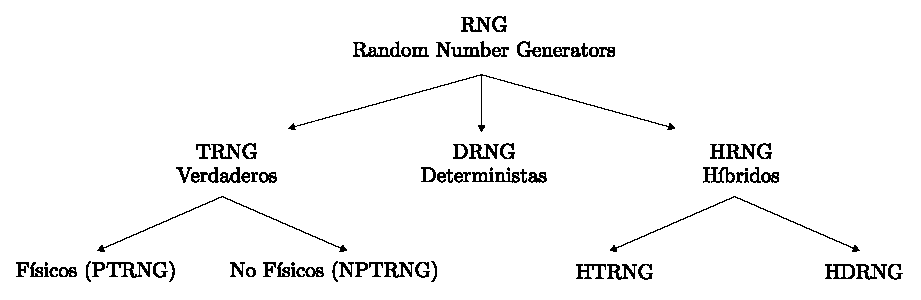
\includegraphics[width=1.0\textwidth]{K0_clasificacion}
	    \caption{Clasificación de los RNG.}
        \label{fig:K0_clasificacion}
    \end{figure}
\end{frame}


% Slide
\begin{frame}
    \frametitle{Generadores de números aleatorios (RNGs)}
    \begin{block}{Parámetros de evaluación}
        \justifying
		\begin{itemize}
		    \item Parámetros relacionados con la calidad
		        \begin{itemize}
		            \item Fuente de aleatoriedad.
		            \item Método de extracción de aleatoriedad y entropía del ruido digital.
		            \item Método de postprocesamiento (opcional).
		            \item Tasa de bits de salida y su estabilidad.
		        \end{itemize}
		    \item Parámetros relacionados con la seguridad
		        \begin{itemize}
		            \item Existencia de un modelo matemático.
		            \item Comprobabilidad interna.
		            \item Seguridad (robustez, resistencia contra ataques).
		        \end{itemize}
		    \item Parámetros relacionados con el diseño
		        \begin{itemize}
		            \item El uso de recursos.
		            \item El consumo de energía.
		            \item Viabilidad en dispositivos lógicos y FPGAs.
		            \item Automatización del diseño.
		        \end{itemize}
		\end{itemize}   
		\vspace{0.1cm}
	\end{block}
\end{frame}

% Slide
\begin{frame}
    \frametitle{Generadores de números aleatorios (RNGs)}
    \begin{block}{Fuentes de aleatoriedad}
        \justifying
        Los fenómenos físicos más utilizados para generar números aleatorios en los dispositivos lógicos son:
        
        \begin{itemize}
            \item[•] Señales analógicas (ruido térmico).
            \item[•] Metaestabilidad.
            \item[•] Jitter del reloj.
            \item[•] Caos.
        \end{itemize}
	\end{block}
\end{frame}


% Slide
\begin{frame}
    \frametitle{Generadores de números aleatorios (RNGs)}
    \begin{block}{Jitter}
        \justifying
         Es una variación del flanco del reloj desde su posición ideal o la incertidumbre en la oscilación del reloj en el dominio del tiempo.
	\end{block}
	\begin{figure}[hbtp]
        \centering
        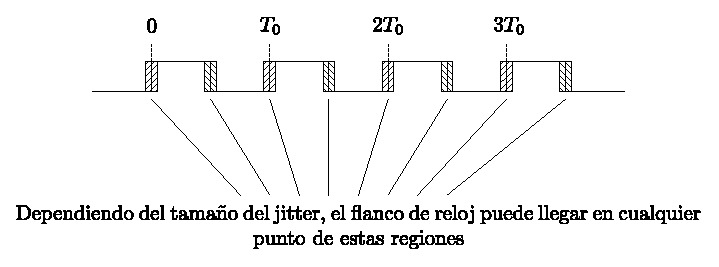
\includegraphics[width=0.9\textwidth]{F9_jitter}
        \caption{Jitter del reloj.}
        \label{fig:F9_jitter}
    \end{figure}
\end{frame}


% Slide
\begin{frame}
    \frametitle{Generadores de números aleatorios (RNGs)}
    \begin{block}{Jitter}
        \justifying
         Los circuitos digitales utilizan un nivel de referencia para detectar los flancos de reloj. Este nivel de referencia debe ser más estable posible. En la práctica sufre fluctuaciones debido a diversos tipos de ruido. Cuando el nivel de referencia se desplaza, los flancos del reloj se detectan antes o después de lo previsto, lo que resulta en una variación temporal conocida como jitter de reloj.
	\end{block}
    \begin{figure}[hbtp]
        \centering
        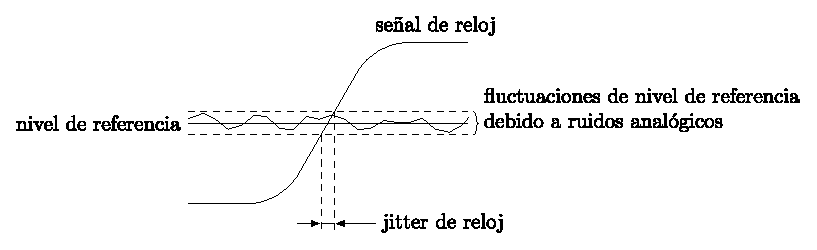
\includegraphics[width=0.8\textwidth]{F10_fluctuaciones}
        \caption{Fluctuaciones del nivel de referencia originadas por ruidos analógicos que provocan jitter del reloj en los circuitos digitales. \cite{Petura2019}}
        \label{fig:F10_fluctuaciones}
    \end{figure}
\end{frame}



% Slide
\begin{frame}
    \frametitle{Generadores de números aleatorios (RNGs)}
    \begin{block}{Núcleos TRNG en FPGA}
        \justifying
        Con base en los criterios del AIS-20/31 \cite{Petura2016}, los núcleos TRNG adecuados para utilizarse en dispositivos lógicos programables (FPGA) que usan estructuras oscilantes son:
		\begin{itemize}
            \item Elementary ring oscillator based TRNG (ERO-TRNG).
            \item Coherent sampling ring oscillator based TRNG (COSO-TRNG).
            \item Multi-ring oscillator based TRNG (MURO-TRNG).
            \item Transient effect ring oscillator based TRNG (TERO-TRNG).
            \item Self-timed ring based TRNG  (STR-TRNG).
            \item Phase-locked loop based TRNG (PLL-TRNG).
        \end{itemize}  
	\end{block}
\end{frame}


% Slide
\begin{frame}
    \frametitle{Generadores de números aleatorios (RNGs)}
    \begin{block}{Núcleo ERO-TRNG, Elementary ring oscillator based TRNG}
        \justifying
         Se propuso y modeló en \cite{Baudet2010}. Dos osciladores de anillo idénticos forman la base del generador. Uno de ellos se utiliza para muestrear la salida del otro oscilador en anillo utilizando un flip-flop D. La frecuencia del oscilador de anillo de muestreo se divide por $K$ para obtener una frecuencia más baja de la señal de muestreo, lo que permitiría acumular el jitter del oscilador de anillo muestreado.
	\end{block}
	\begin{figure}[hbtp]
	    \centering
	    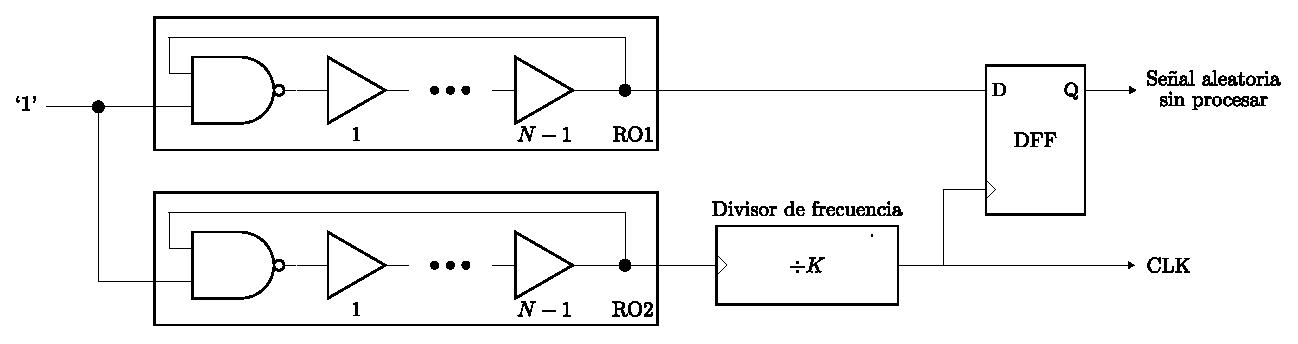
\includegraphics[width=0.8\textwidth]{A1_ERO_TRNG}
	    \caption{Diagrama de ERO-TRNG.}
        \label{fig:A1_ERO_TRNG}
    \end{figure}
\end{frame}

% Slide
\begin{frame}
    \frametitle{Generadores de números aleatorios (RNGs)}
    \begin{block}{Ventajas y desventajas del núcleo ERO-TRNG}
        \justifying
          \begin{figure}[!h]
				\begin{minipage}[t]{0.48\textwidth}
					\textbf{Ventajas}
					\begin{itemize}
						\justifying
						\item Implementación sencilla.
						\item Repetible sin intervención manual.
						\item Sólido modelo estocástico.
						\item Bajo consumo de potencia.
					\end{itemize}
				\end{minipage} \hfill \begin{minipage}[t]{0.48\textwidth}
					\textbf{Desventajas}
					\begin{itemize}
						\justifying
						\item Tasa de bits de salida relativamente baja.
					\end{itemize}
				\end{minipage}
			\end{figure}		
	\end{block}
\end{frame}


% Slide
\begin{frame}
    \frametitle{Generadores de números aleatorios (RNGs)}
    \begin{block}{Núcleo COSO-TRNG, Coherent sampling ring oscillator based TRNG}
        \justifying
         Se propuso por primera vez en \cite{Kohlbrenner2004}. Utiliza dos osciladores de anillo idénticos como fuente de aleatoriedad. Las frecuencias de los osciladores varían un poco. Al muestrear la salida de uno de los osciladores mediante un flip-flop D sincronizado con la salida del otro oscilador, se obtiene una señal con un periodo variable, que corresponde al desfase relativo de los dos osciladores.
	\end{block}
	\begin{figure}[hbtp]
	    \centering
	    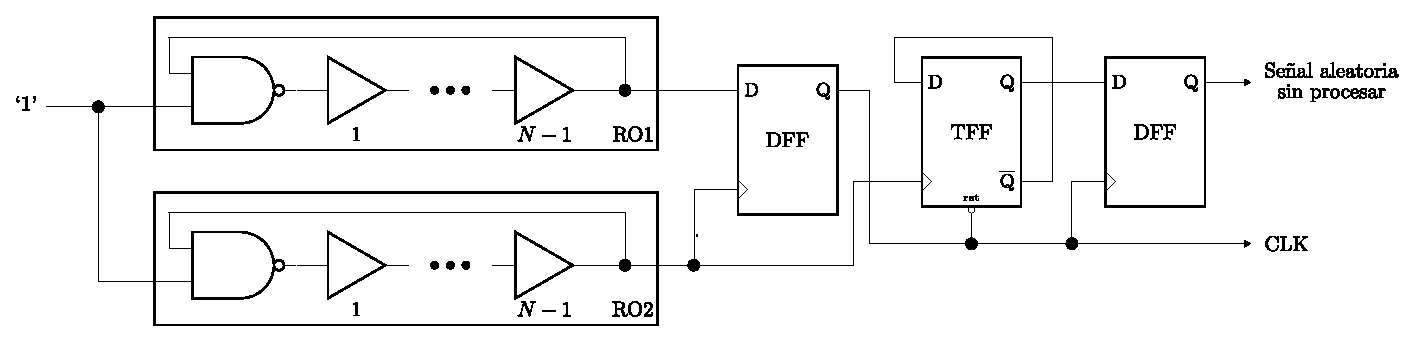
\includegraphics[width=0.8\textwidth]{A2_COSO_TRNG}
	    \caption{Diagrama de COSO-TRNG.}
        \label{fig:A2_COSO_TRNG}
    \end{figure}
\end{frame}

% Slide
\begin{frame}
    \frametitle{Generadores de números aleatorios (RNGs)}
    \begin{block}{Ventajas y desventajas del núcleo COSO-TRNG}
        \justifying
          \begin{figure}[!h]
				\begin{minipage}[t]{0.48\textwidth}
					\textbf{Ventajas}
					\begin{itemize}
						\justifying
						\item Ocupa un área muy pequeña.
						\item Tasa de bits de salida relativamente alta.
						\item Bajo consumo de potencia.
					\end{itemize}
				\end{minipage} \hfill \begin{minipage}[t]{0.48\textwidth}
					\textbf{Desventajas}
					\begin{itemize}
						\justifying
						\item Implementación difícil.
						\item Requiere intervención manual.
					\end{itemize}
				\end{minipage}
			\end{figure}		
	\end{block}
\end{frame}


% Slide
\begin{frame}
    \frametitle{Generadores de números aleatorios (RNGs)}
    \begin{block}{Núcleo MURO-TRNG, Multi-ring oscillator based TRNG}
        \justifying
        Se propuso por primera vez en \cite{Sunar2007}. Utiliza $m$ osciladores en anillo como fuente de aleatoriedad. Los osciladores deben ser independientes y su fase uniformemente distribuida. Para extraer la aleatoriedad el número de osciladores de anillo debe satisfacer $m > T/\sigma $ donde $T$ es el valor medio del periodo de reloj y $\sigma$ es la desviación típica del jitter acumulado durante el periodo de muestreo.
	\end{block}
	\begin{figure}[hbtp]
	    \centering
	    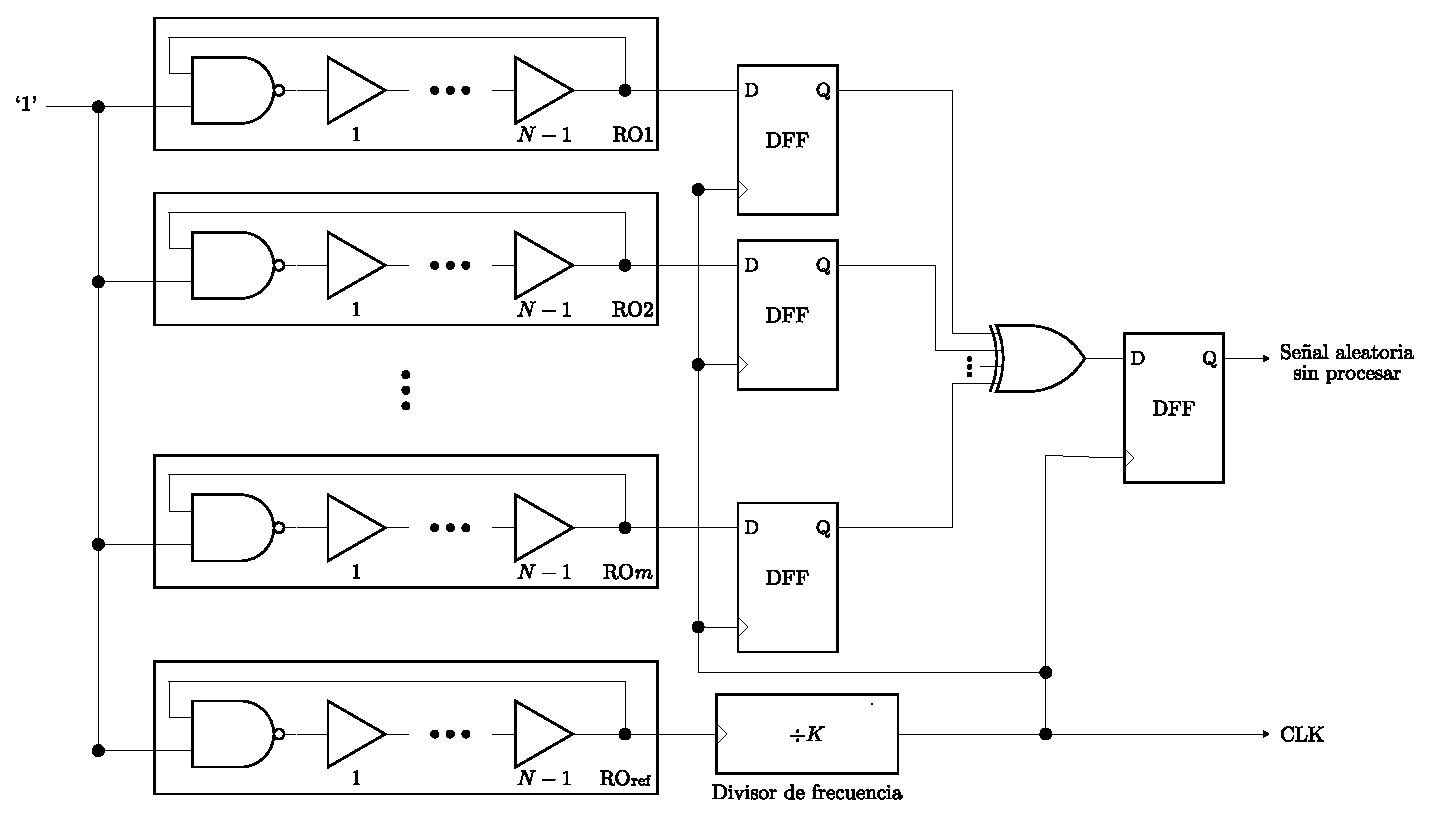
\includegraphics[width=0.5\textwidth]{A3_MURO_TRNG}
	    \caption{Diagrama de MURO-TRNG.}
        \label{fig:A3_MURO_TRNG}
    \end{figure}
\end{frame}


% Slide
\begin{frame}
    \frametitle{Generadores de números aleatorios (RNGs)}
    \begin{block}{Ventajas y desventajas del núcleo MURO-TRNG}
        \justifying
          \begin{figure}[!h]
				\begin{minipage}[t]{0.48\textwidth}
					\textbf{Ventajas}
					\begin{itemize}
						\justifying
						\item No requiere intervención manual.
						\item Tasa de bits relativamente alta.
					\end{itemize}
				\end{minipage} \hfill \begin{minipage}[t]{0.48\textwidth}
					\textbf{Desventajas}
					\begin{itemize}
						\justifying
						\item Ocupa un área muy grande.
						\item Los osciladores de anillo pueden bloquearse entre sí.
						\item Alto consumo de potencia.
					\end{itemize}
				\end{minipage}
			\end{figure}		
	\end{block}
\end{frame}


% Slide
\begin{frame}
    \frametitle{Generadores de números aleatorios (RNGs)}
    \begin{block}{Núcleo TERO-TRNG, Transient effect ring oscillator based TRNG}
        \justifying
         Se propuso en \cite{Varchola2010} y el modelo estocástico en \cite{Haddad2015}. Genera bits aleatorios utilizando metaestabilidad oscilatoria. Debido a la metaestabilidad oscilatoria del TERO, el número de oscilaciones es aleatorio. Para producir un flujo de bits aleatorios, el TERO debe reiniciarse periódicamente
	\end{block}
	\begin{figure}[hbtp]
	    \centering
	    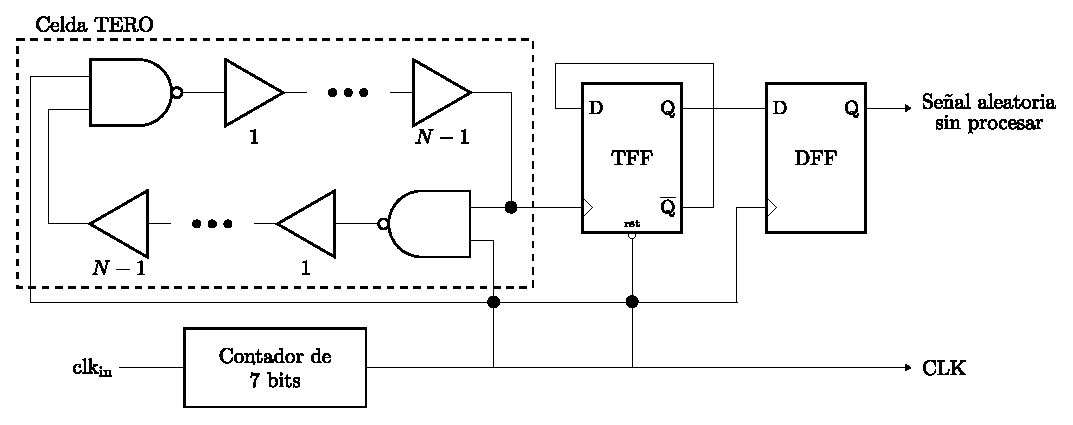
\includegraphics[width=0.7\textwidth]{A4_TERO_TRNG}
	    \caption{Diagrama de TERO-TRNG.}
        \label{fig:A4_TERO_TRNG}
    \end{figure}
\end{frame}


% Slide
\begin{frame}
    \frametitle{Generadores de números aleatorios (RNGs)}
    \begin{block}{Ventajas y desventajas del núcleo TERO-TRNG}
        \justifying
          \begin{figure}[!h]
				\begin{minipage}[t]{0.48\textwidth}
					\textbf{Ventajas}
					\begin{itemize}
						\justifying
						\item Ocupa un área muy pequeña.
						\item Tasa de bits relativamente alta.
						\item Bajo consumo de potencia.
					\end{itemize}
				\end{minipage} \hfill \begin{minipage}[t]{0.48\textwidth}
					\textbf{Desventajas}
					\begin{itemize}
						\justifying
						\item Requiere intervención manual.
						\item No es repetible.
					\end{itemize}
				\end{minipage}
			\end{figure}		
	\end{block}
\end{frame}

% Slide
\begin{frame}
    \frametitle{Generadores de números aleatorios (RNGs)}
    \begin{block}{Núcleo STR-TRNG, Self-timed ring based TRNG}
        \justifying
         Se propuso en \cite{Cherkaoui2013}. Se compone de $L$ celdas Muller. El principio de extracción de aleatoriedad de un STR-TRNG es el mismo que el de MURO-TRNG. El reloj de muestreo se genera mediante un oscilador en anillo. La ventaja de un STR es que, si se configura correctamente, garantiza que las fases del reloj de salida estén igualmente espaciadas
	\end{block}
	\begin{figure}[hbtp]
	    \centering
	    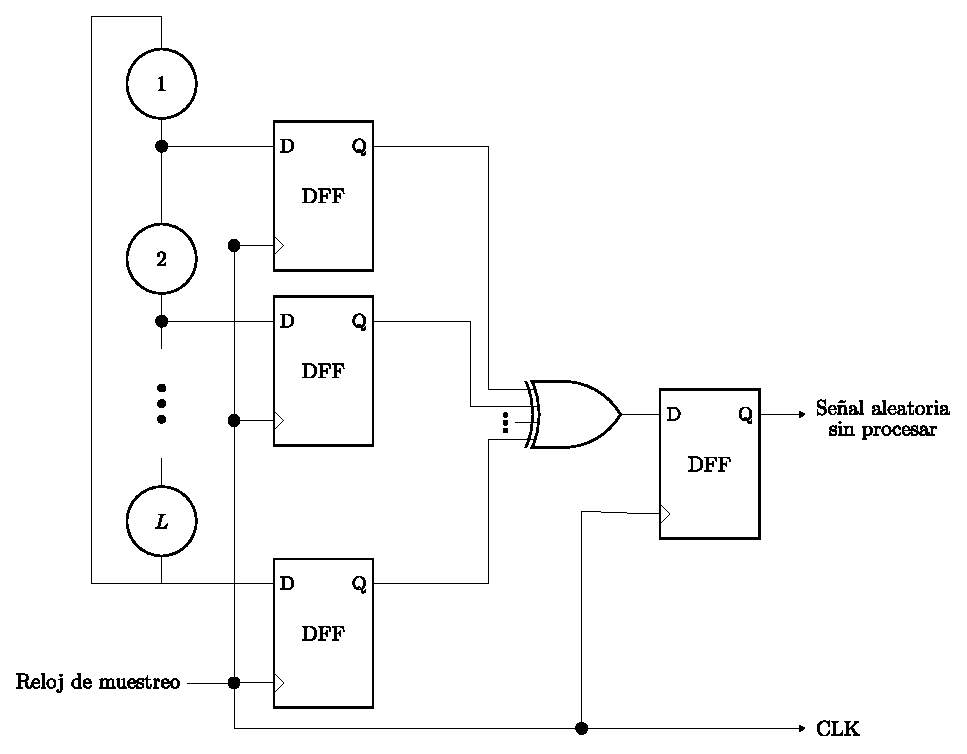
\includegraphics[width=0.4\textwidth]{A5_STR_TRNG}
	    \caption{Diagrama de STR-TRNG.}
        \label{fig:A5_STR_TRNG}
    \end{figure}
\end{frame}


% Slide
\begin{frame}
    \frametitle{Generadores de números aleatorios (RNGs)}
    \begin{block}{Ventajas y desventajas del núcleo STR-TRNG}
        \justifying
          \begin{figure}[!h]
				\begin{minipage}[t]{0.48\textwidth}
					\textbf{Ventajas}
					\begin{itemize}
						\justifying
						\item La tasa de bits es muy alta.
					\end{itemize}
				\end{minipage} \hfill \begin{minipage}[t]{0.48\textwidth}
					\textbf{Desventajas}
					\begin{itemize}
						\justifying
						\item Ocupa un área muy grande.
						\item Requiere intervención manual.
						\item Alto consumo de potencia.
					\end{itemize}
				\end{minipage}
			\end{figure}		
	\end{block}
\end{frame}

% Slide
\begin{frame}
    \frametitle{Generadores de números aleatorios (RNGs)}
    \begin{block}{Núcleo PLL-TRNG, Phase-locked loop based TRNG}
        \justifying
        Se propuso en \cite{Fischer2003}. El generador se basa en el hecho de que utilizando PLLs, las frecuencias de dos relojes generados están mutuamente relacionadas. La elección de los parámetros del PLL no es trivial. Hay que respetar muchas restricciones, incluidas las físicas del fabricante del PLL y las de seguridad del TRNG.
	\end{block}
	\begin{figure}[hbtp]
	    \centering
	    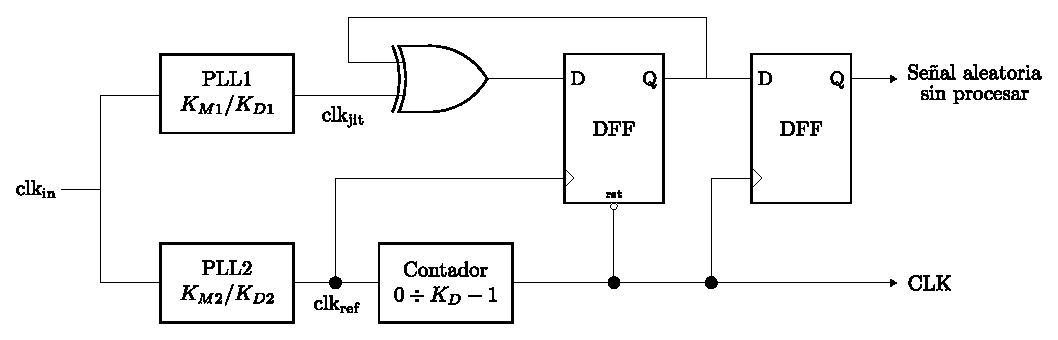
\includegraphics[width=0.7\textwidth]{A6_PLL_TRNG}
	    \caption{Diagrama de PLL-TRNG.}
        \label{fig:A6_PLL_TRNG}
    \end{figure}
\end{frame}

% Slide
\begin{frame}
    \frametitle{Generadores de números aleatorios (RNGs)}
    \begin{block}{Ventajas y desventajas del núcleo PLL-TRNG}
        \justifying
          \begin{figure}[!h]
				\begin{minipage}[t]{0.48\textwidth}
					\textbf{Ventajas}
					\begin{itemize}
						\justifying
						\item No requiere intervención manual.
						\item Es repetible.
						\item Ocupa un área relativamente pequeña.
						\item La tasa de bits es relativamente alta.
					\end{itemize}
				\end{minipage} \hfill \begin{minipage}[t]{0.48\textwidth}
					\textbf{Desventajas}
					\begin{itemize}
						\justifying
						\item Consumo de potencia medio.
						\item Diferencias entre familias de FPGAs.
					\end{itemize}
				\end{minipage}
			\end{figure}		
	\end{block}
\end{frame}

% Slide
\begin{frame}
    \frametitle{Generadores de números aleatorios (RNGs)}
    \begin{block}{Núcleos TRNG en FPGA}
        \justifying
\begin{table}[htbp]
  \centering
    \caption{Resumen de los resultados núcleos TRNGs \cite{Petura2016}.}
    \resizebox{0.9\linewidth}{!}{ 
        \begin{tabular}{|c|c|c|c|c|c|c|c|c|}
            \hline
            \rowcolor{lightgray} TRNG Type & FPGA  & Area  & Power cons. & Bit Rate & Efficiency & Entropy & Entropy * Bit rate & Feasib. \\
            \rowcolor{lightgray}       & device & (LUT/Reg) & [mW]  & [Mbits/s] & [bits/$\mu$Ws] & per bit &       & \& Repeat. \\
            \hline
            \multirow{3}[2]{*}{ERO} & Spartan 6 & 46/19 & 2.16  & 0.0042 & 1.94  & 0.999 & 0.004 & \multirow{3}[2]{*}{5} \\
                  & Cyclone V & 34/20 & 3.24  & 0.0027 & 0.83  & 0.990 & 0.003 &  \\
                  & SmartFusion 2 & 45/19 & 4     & 0.014 & 3.5   & 0.980 & 0.013 &  \\
            \hline
            \multirow{3}[2]{*}{COSO} & Spartan 6 & 18/3  & 1.22  & 0.54  & 442.6 & 0.999 & 0.539 & \multirow{3}[2]{*}{1} \\
                  & Cyclone V & 13/3  & 0.9   & 1.44  & 1600  & 0.999 & 1.438 &  \\
                  & SmartFusion 2 & 23/3  & 1.94  & 0.328 & 169   & 0.999 & 0.327 &  \\
            \hline
            \multirow{3}[2]{*}{MURO} & Spartan 6 & 521/131 & 54.72 & 2.57  & 46.9  & 0.999 & 2.567 & \multirow{3}[2]{*}{4} \\
                  & Cyclone V & 525/130 & 34.93 & 2.2   & 62.9  & 0.999 & 2.197 &  \\
                  & SmartFusion 2 & 545/130 & 66.41 & 3.62  & 54.5  & 0.999 & 3.616 &  \\
            \hline
            \multirow{3}[2]{*}{PLL} & Spartan 6 & 34/14 & 10.6  & 0.44  & 41.5  & 0.981 & 0.431 & \multirow{3}[2]{*}{3} \\
                  & Cyclone V & 24/14 & 23    & 0.6   & 43.4  & 0.986 & 0.592 &  \\
                  & SmartFusion 2 & 30/15 & 19.7  & 0.37  & 18.7  & 0.921 & 0.340 &  \\
            \hline
            \multirow{3}[2]{*}{TERO} & Spartan 6 & 39/12 & 3.312 & 0.625 & 188.7 & 0.999 & 0.624 & \multirow{3}[2]{*}{1} \\
                  & Cyclone V & 46/12 & 9.36  & 1     & 106.8 & 0.987 & 0.985 &  \\
                  & SmartFusion 2 & 46/12 & 1.23  & 1     & 813   & 0.999 & 0.999 &  \\
            \hline
            \multirow{3}[2]{*}{STR} & Spartan 6 & 346/256 & 65.9  & 154   & 2343.2 & 0.998 & 154.121 & \multirow{3}[2]{*}{2} \\
                  & Cyclone V & 352/256 & 49.4  & 245   & 4959.1 & 0.999 & 244.755 &  \\
                  & SmartFusion 2 & 350/256 & 82.52 & 188   & 2286.7 & 0.999 & 188.522 &  \\
            \hline
        \end{tabular}%
    }
  \label{tab:resumen_de_trng_cores}
\end{table}%
   
	\end{block}
\end{frame}

\section{Mapa caótico}

% Slide
\begin{frame}
    \frametitle{Mapa caótico}
    \begin{block}{Definición de mapa caótico}
        \justifying
        Los mapas caóticos, mapas iterados, ecuaciones de diferencias o simplemente mapas, son sistemas dinámicos en tiempo discreto que tienen la forma general $x_{n+1} = f(x_{n})$, los cuales requieren una condición inicial $x_{0}$ y se iteran continuamente para conocer su comportamiento. A la secuencia $x_{0}, x_{1}, x_{2} , \ldots $ se le conoce como la órbita del mapa comenzando desde $x_{0}$.
	\end{block}
	
	\begin{figure}[hbtp]
            \centering
            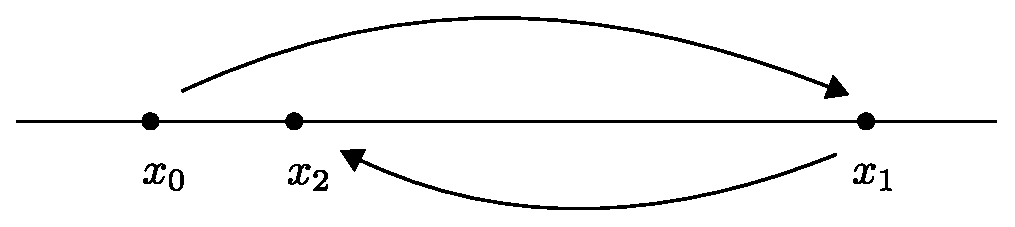
\includegraphics[width=0.7\textwidth]{F0_mapdiagram}
            \caption{Ejemplo de mapeo en una dimensión.}
            \label{fig:F0_mapdiagram}
        \end{figure}
\end{frame}


% Slide
\begin{frame}
    \frametitle{Mapa caótico}
    \begin{block}{Mapa caótico bidimensional}
        \justifying
        En el artículo \cite{Sprott1993} se analiza y estudia el mapa caótico cuadrático bidimensional más sencillo que esta dado por:
        \begin{equation}
            \begin{array}{ccl}
                x_{n+1} & = &  a_{1} + a_{2}x_{n} + a_{3}x_{n}^{2} + a_{4}x_{n}y_{n} + a_{5}y_{n} + a_{6}y_{n}^{2}\\
                y_{n+1} & = &  a_{7} + a_{8}x_{n} + a_{9}x_{n}^{2} + a_{10}x_{n}y_{n} + a_{11}y_{n} + a_{12}y_{n}^{2}
            \end{array}
            \label{eq:mapa_caotico}
	    \end{equation}
	     donde los parámetros $\{a_{1}, a_{2}, \ldots a_{12}\}$ y las condiciones iniciales $x_{0}$ y $y_{0}$ determinan las características de la solución. La iteraciones se representan como puntos en una superficie bidimensional. Requiere de 10 sumas y 13 multiplicaciones. 
	\end{block}
\end{frame}

% Slide
\begin{frame}
    \frametitle{Mapa caótico}
    \begin{block}{Comportamiento del mapa}
        \justifying
         La iteraciones se representan como puntos en una superficie bidimensional. Después de un cierto número de iteraciones, la solución hará una de estas cuatro cosas: 
            \begin{itemize}
                \item[(a)] convergerá a un único punto fijo.
                \item[(b)] tomará una sucesión de valores que acabarán repitiéndose, produciendo un ciclo límite.
                \item[(c)] será inestable y divergirá hasta el infinito.
                \item[(d)] mostrará caos y rellenará gradualmente alguna región a menudo complicada pero acotada del plano $x-y$.
            \end{itemize}                     
	\end{block}
\end{frame}

% Slide
\begin{frame}
    \frametitle{Mapa caótico}
    \begin{block}{Pasos para encontrar atractores}
        \justifying
         Para saber qué valores de $\{a_{1}, a_{2}, \ldots a_{12}\}$ llevan al caos, \cite{Sprott1993} utilizó el siguiente procedimiento.

        \begin{enumerate}
            \item Elegir aleatoriamente los 12 coeficientes de $a_{1}$ hasta $a_{12}$ aleatoriamente sobre algún intervalo.
            \item Elegir las condiciones iniciales $x_{0}$ y $y_{0}$.
            \item Iterar las ecuaciones del mapa mientras se calcula el exponente de Lyapunov y se comprueba si no hay divergencia.
            \item Mantener las soluciones que están acotadas y tienen un exponente de Lyapunov positivo.
        \end{enumerate}              
	\end{block}
\end{frame}


% Slide
\begin{frame}
    \frametitle{Mapa caótico}
    \begin{block}{Codificación y rango de búsqueda}
        \justifying
        \begin{itemize}
            \item Los coeficientes seleccionados en incrementos de 0.1 en el intervalo de $-1.2$ a $1.2$, es decir, 25 valores posibles.
            \item Codificación con letras del alfabeto $A$ hasta la $Y$.
            \item  $A = -1.2, B = -1.1, C = -1.0, \ldots, Y = 1.2$.
            \item Cada atractor se identifica unívocamente con un nombre de 12 letras.
            \item El número de posibles casos es $25^{12}$ o aproximadamente $6\times 10^{12}$.
            \item Aproximadamente 1.6\% son caóticos.
        \end{itemize}      
	\end{block}
\end{frame}

% Slide
\begin{frame}
    \frametitle{Mapa caótico}
    \begin{block}{Codificación de parámetros $a_{n}$}
        \justifying 
        \begin{table}[htbp]
            \centering
            \caption{Conversiones para codificación de los atractores.}
            \resizebox{0.5\linewidth}{!}{
            \begin{tabular}{|l|l|l|l|}
                \hline
                \rowcolor{lightgray}   Letra & Codificación & Letra & Codificación\\
                A & -1.2 & N & 0.1 \\ 
                \hline
                B & -1.1 & O & 0.2 \\ 
                \hline
                C & -1.0 & P & 0.3 \\ 
                \hline
                D & -0.9 & Q & 0.4 \\ 
                \hline
                E & -0.8 & R & 0.5 \\ 
                \hline
                F & -0.7 & S & 0.6 \\ 
                \hline
                G & -0.6 & T & 0.7 \\ 
                \hline
                H & -0.5 & U & 0.8 \\ 
                \hline
                I & -0.4 & V & 0.9 \\ 
                \hline
                J & -0.3 & W & 1.0 \\ 
                \hline
                K & -0.2 & X & 1.1 \\ 
                \hline
                L & -0.1 & Y & 1.2 \\ 
                \hline
                M & -0.0 &   &     \\ 
                \hline
            \end{tabular}
            }
            \label{tab:conversion_mapas}
        \end{table}
            
	\end{block}
\end{frame}


% Slide
\begin{frame}
    \frametitle{Mapa caótico}
    \begin{block}{Ejemplos de atractores}
        \justifying 
        
         \begin{table}[htbp]
            \centering
            \caption{Diversos identificadores, dimensión fractal y exponente de Lyapunov para atractores del mapa caótico bidimensional.}
            \resizebox{0.9\linewidth}{!}{
            \begin{tabular}{|l|l|l|l|}
                \hline
                \rowcolor{lightgray}  Atractor & Identificador & Dimensión fractal & Exponente de Lyapunov \\
                \hline
                1     & \texttt{GLXOESFTTPSV} & 1.77  & 0.12   \\ %e
                \hline
                2     & \texttt{CVQKGHQTPHTE} & 1.79  & 0.14   \\ %b
                \hline
                3     & \texttt{UWACXDQIGKHF} & 1.42  & 0.10   \\ %n
    \hline
                4    &  \texttt{GIIETPIQRRUL} & 1.50  & 0.13   \\ %d
                \hline
            \end{tabular}
            }
            \label{tab:codificacion}
        \end{table}
	\end{block}
\end{frame}


% Slide
\begin{frame}
    \frametitle{Mapa caótico}
    \begin{block}{Decodificación de parámetros de $a_{n}$ para generar diferentes atractores}
        \justifying
        Después de decodificar los identificadores  tenemos:
        \begin{footnotesize}
            \begin{equation*}
             \begin{array}{lcl}
                A_{1} & = & \{ -0.6, -0.1, \phantom{-}1.1, \phantom{-}0.2, -0.8, \phantom{-}0.6, -0.7, \phantom{-}0.7, \phantom{-}0.7, \phantom{-}0.3, \phantom{-}0.6, \phantom{-}0.9 \}\\
                A_{2} & = & \{ -1.0, \phantom{-}0.9, \phantom{-}0.4, -0.2, -0.6, -0.5, \phantom{-}0.4, \phantom{-}0.7, \phantom{-}0.3, -0.5, \phantom{-}0.7, -0.8 \}\\
                A_{3} & = &  \{\phantom{-}0.8, \phantom{-}1.0, -1.2, -1.0, \phantom{-}1.1, -0.9, \phantom{-}0.4, -0.4, -0.6, -0.2, -0.5, -0.7 \}\\
                A_{4} & = & \{-0.6, -0.4, -0.4, -0.8, \phantom{-}0.7, \phantom{-}0.3, -0.4, \phantom{-}0.4, \phantom{-}0.5, \phantom{-}0.5, \phantom{-}0.8, -0.1 \}\\
            \end{array}
            \end{equation*}
        \end{footnotesize}
        utilizando las condiciones iniciales:
        \begin{equation}
            x_{0} =  0.05,  y_{0} = 0.05
        \end{equation}
	\end{block}
\end{frame}

% Slide
\begin{frame}
    \frametitle{Mapa caótico}
	\begin{figure}[hbtp]
            \centering
            \caption{Diferentes atractores caóticos del mapa bidimensional $A_{1}$ y $A_{2}$.} 
            \begin{subfigure}[b]{0.475\textwidth}
                \centering
                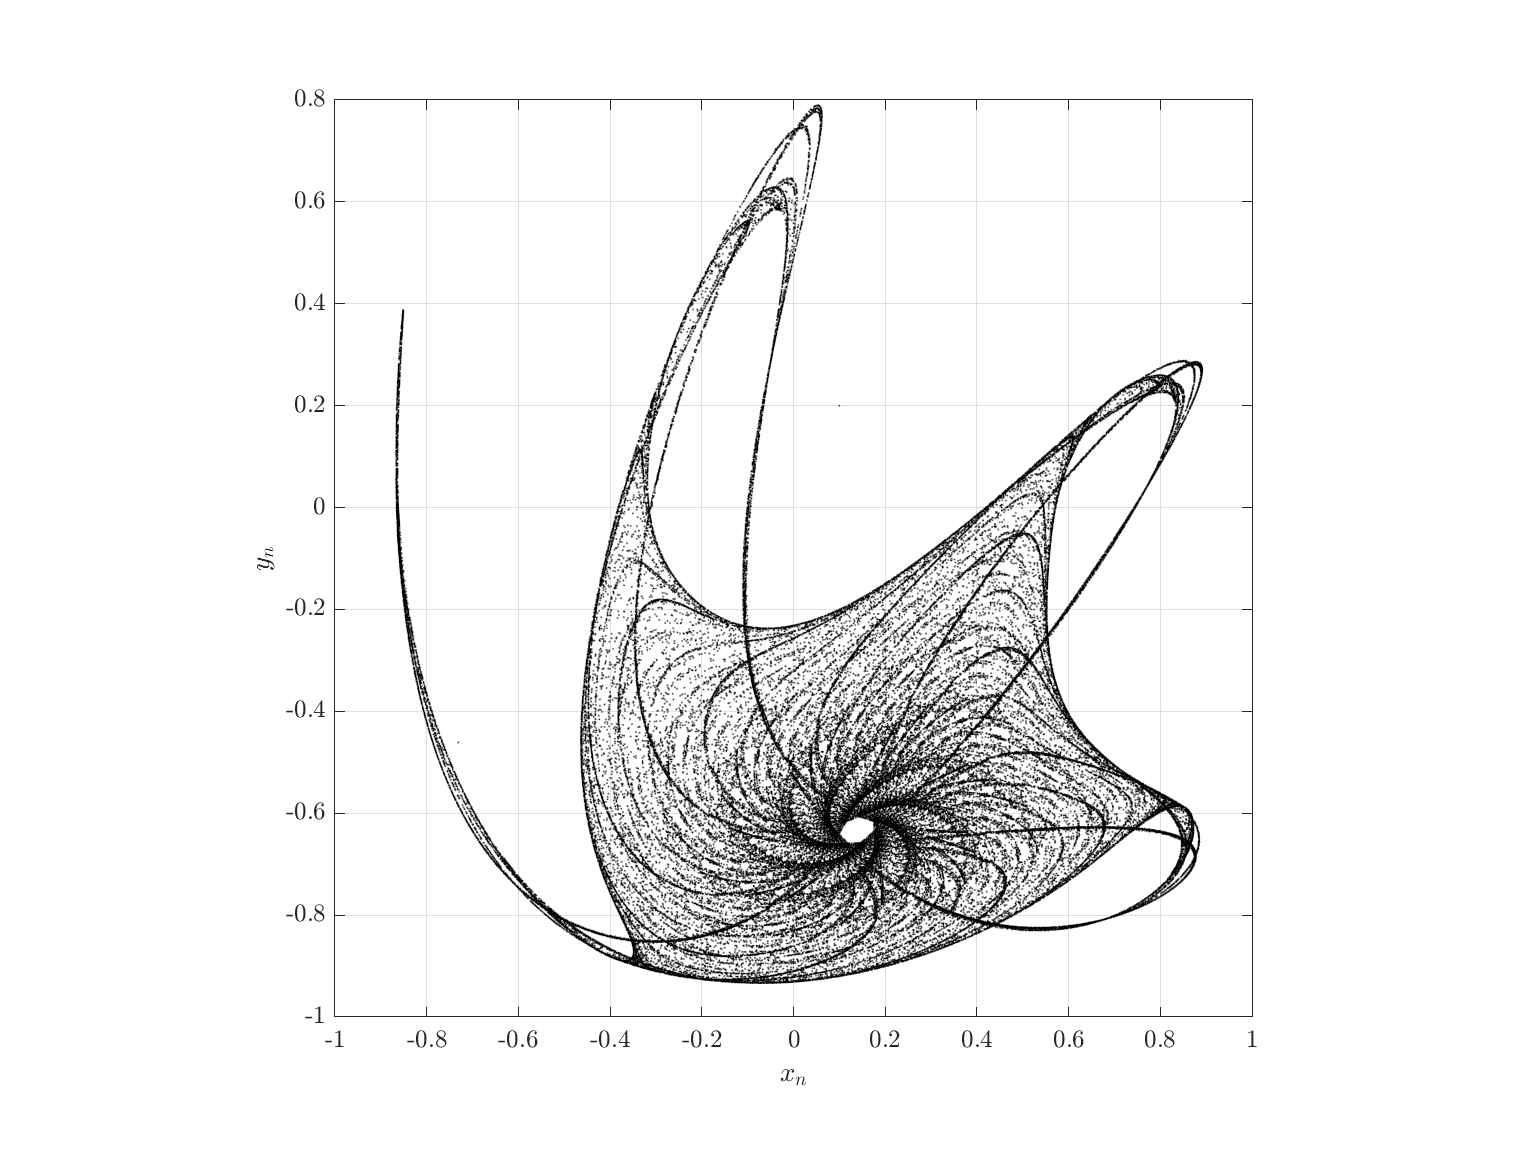
\includegraphics[width=\textwidth,trim=70 0 70 0,clip]{G1_map1}
                \caption{Atractor 1.}    
                \label{fig:mapa_1}
            \end{subfigure}
            \hfill
            \begin{subfigure}[b]{0.475\textwidth}  
                \centering 
                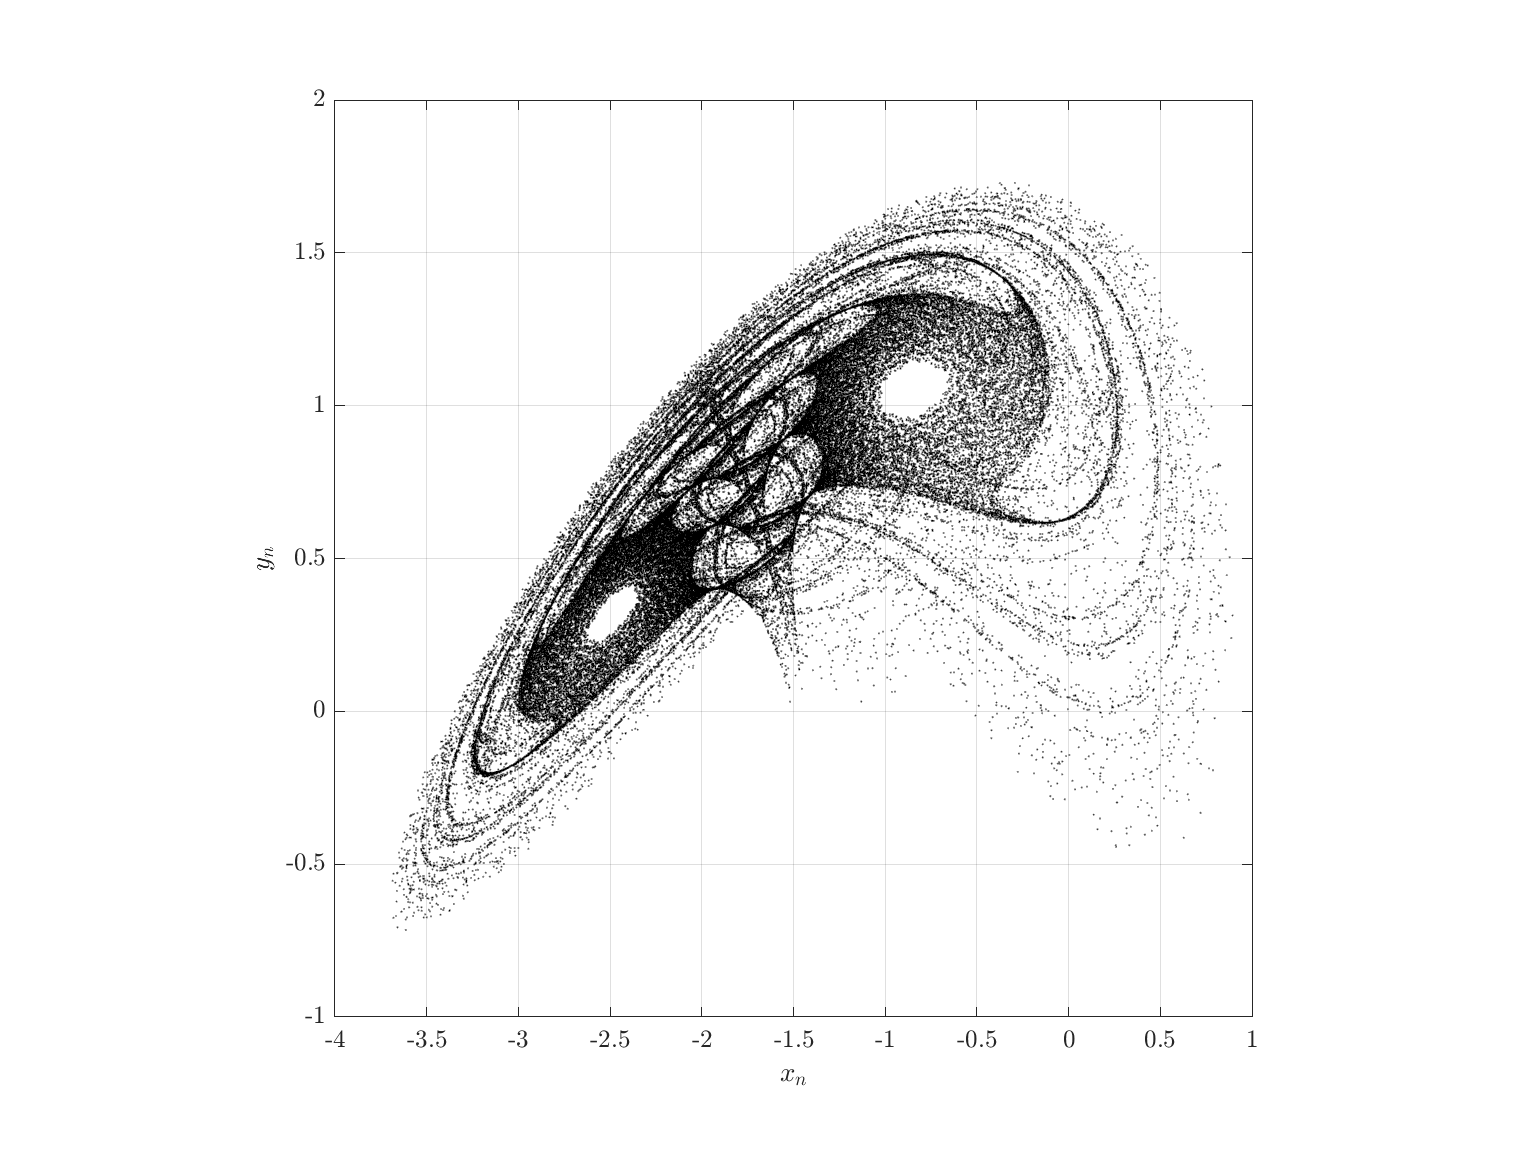
\includegraphics[width=\textwidth,trim=70 0 70 0,clip]{G2_map2}
                \caption{Atractor 2.}    
                \label{fig:mapa_2}
            \end{subfigure}
        \end{figure}
\end{frame}


% Slide
\begin{frame}
    \frametitle{Mapa caótico}
	\begin{figure}[hbtp]
            \centering
            \caption{Diferentes atractores caóticos del mapa bidimensional $A_{3}$ y $A_{4}$.} 
            \begin{subfigure}[b]{0.475\textwidth}   
                \centering 
                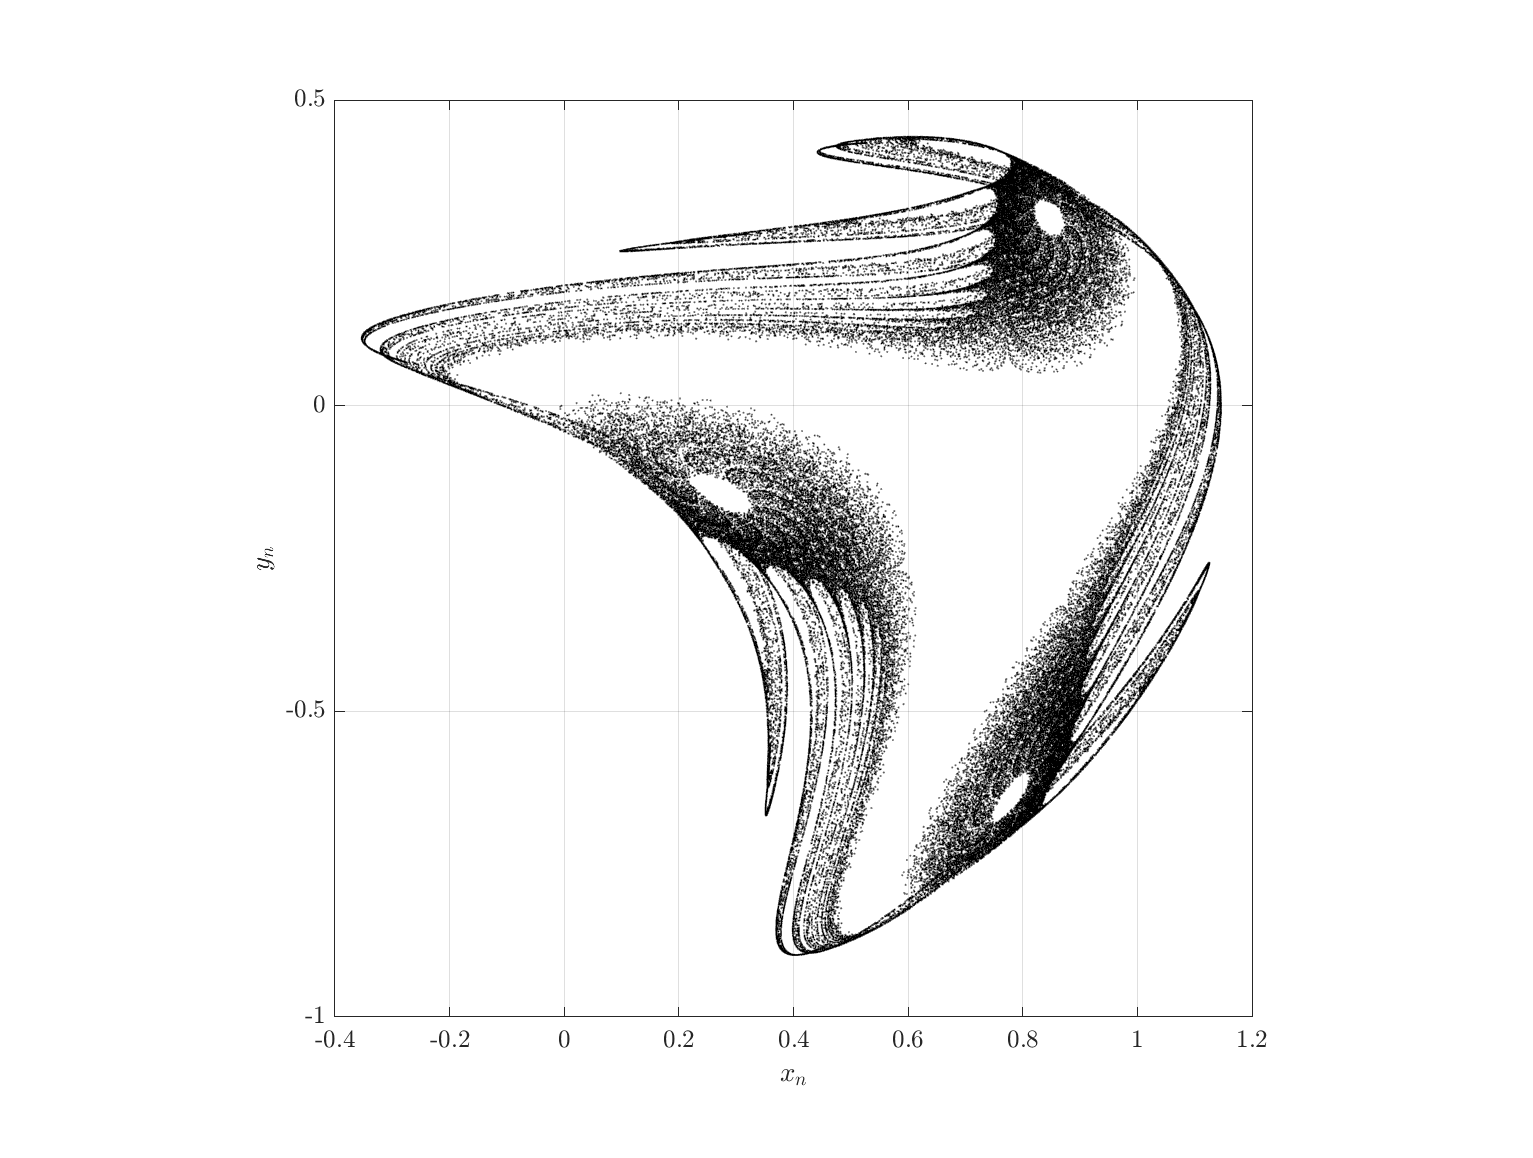
\includegraphics[width=\textwidth,trim=70 0 70 0,clip]{G3_map3}
                \caption{Atractor 3.}    
                \label{fig:mapa_3}
            \end{subfigure}
            \hfill
            \begin{subfigure}[b]{0.475\textwidth}   
                \centering 
                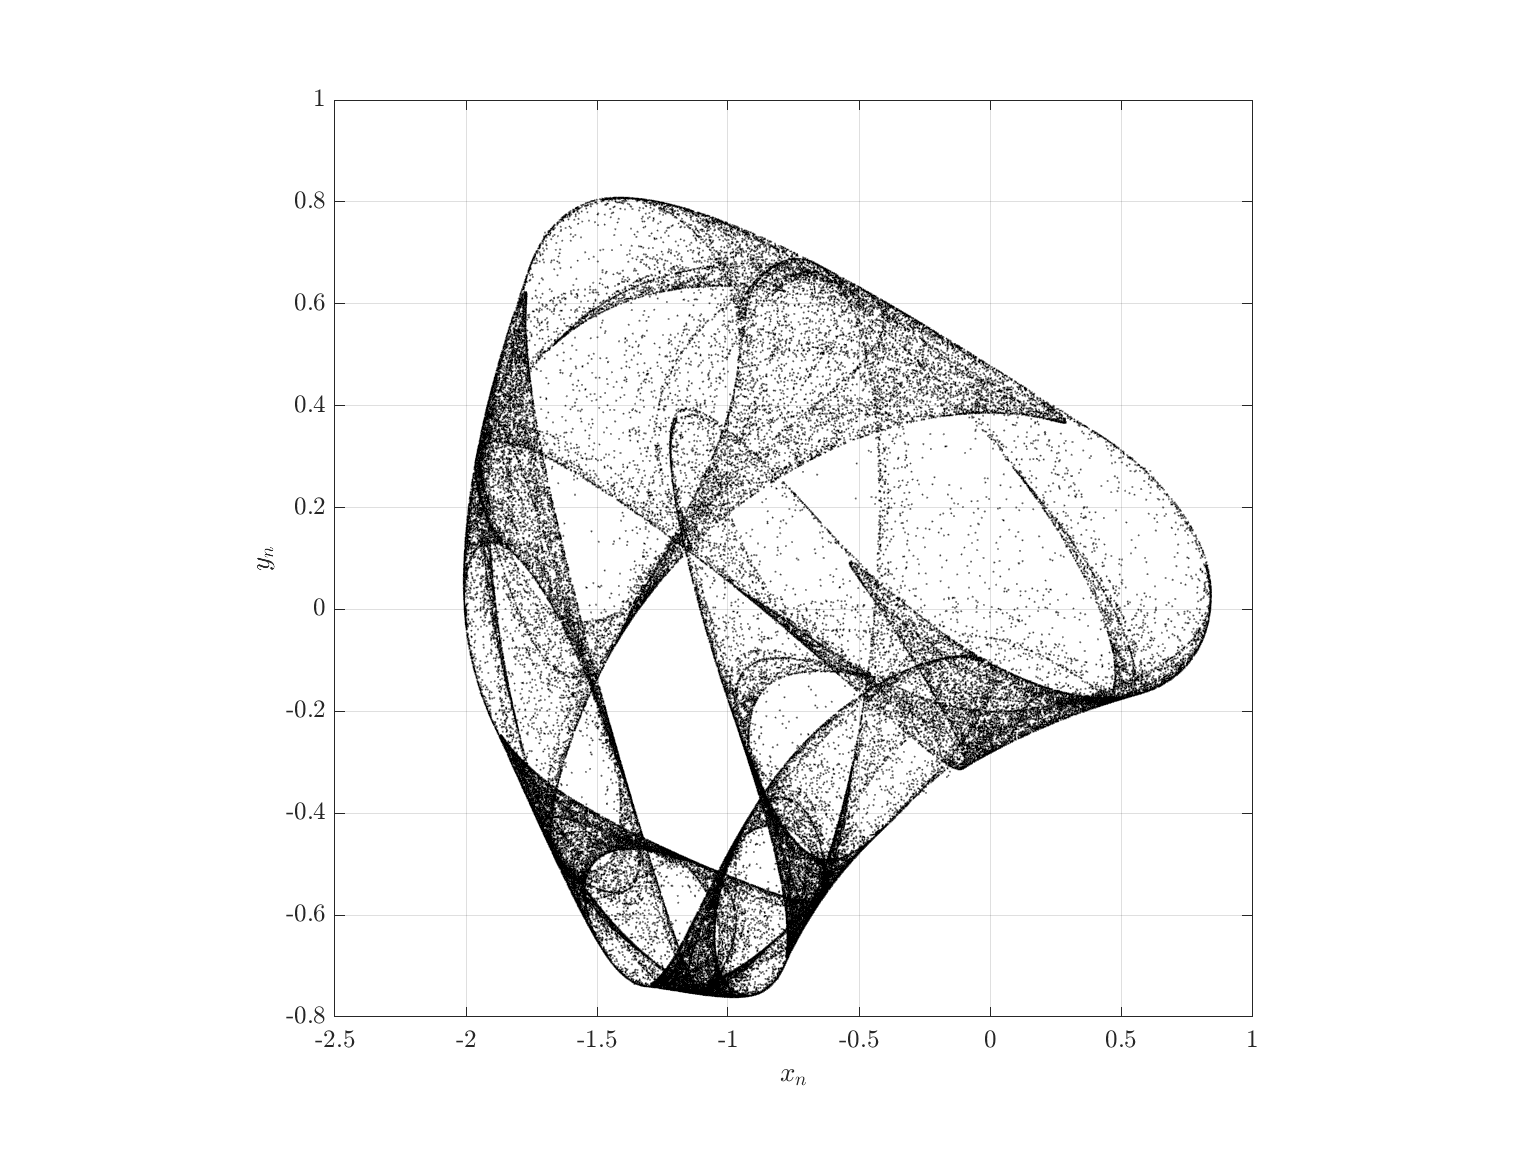
\includegraphics[width=\textwidth,trim=70 0 70 0,clip]{G4_map4}
                \caption{Atractor 4.}    
                \label{fig:mapa_4}
            \end{subfigure}
        \end{figure}
\end{frame}


% Slide
\begin{frame}
    \frametitle{Mapa caótico}
     \begin{block}{¿Qué condiciones iniciales generan caos? - Dominio de atracción}
        \justifying
        \begin{itemize}
            \item No se saben las posibles variaciones que pueden ocurrir al modificar las condición iniciales $x_{0}$ y $y_{0}$.
            \item No se conoce el rango que pueden tener las condiciones iniciales en el que se asegure que exista el caos.
        \end{itemize}
	\end{block}
\end{frame}

% Slide
\begin{frame}
    \frametitle{Mapa caótico}
     \begin{block}{Pasos para calcular dominio de atracción}
        \justifying
        Podemos calcularlo numéricamente siguiendo los siguientes pasos:

        \begin{enumerate}
            \item Elegir un rango para $x_{0} \in [x_{\text{izq}}, x_{\text{der}}]$ y $y_{0} \in [y_{\text{izq}}, y_{\text{der}}]$ y un tamaño de paso $h$ donde se va a realizar el análisis.
            \item Iterar el mapa unos cientos de veces para cada uno de los posibles valores de $x_{0}$ y $y_{0}$ dentro del rango y el tamaño de paso $h$ seleccionado. Para cada combinación almacenar todas las iteraciones en un vector.
            \item Comprobar cada vector en busca de puntos fijos, divergencia y de ser posible ciclos límite.
            \item En una matriz de tamaño, $m \times n$, donde $m$ es el número de elementos en el rango de $y_{0}$ y $n$ el número de elementos del rango de $x_{0}$, escribir 1 si esta dentro del rango que produce caos o $0$ si esta fuera.
        \end{enumerate}
	\end{block}
\end{frame}


% Slide
\begin{frame}
    \frametitle{Mapa caótico}
	\begin{figure}[hbtp]
            \centering
            \caption{Diferentes atractores caóticos y dominios de atracción del mapa bidimensional $A_{1}$ y $A_{2}$.} 
            \begin{subfigure}[b]{0.475\textwidth}
                \centering
                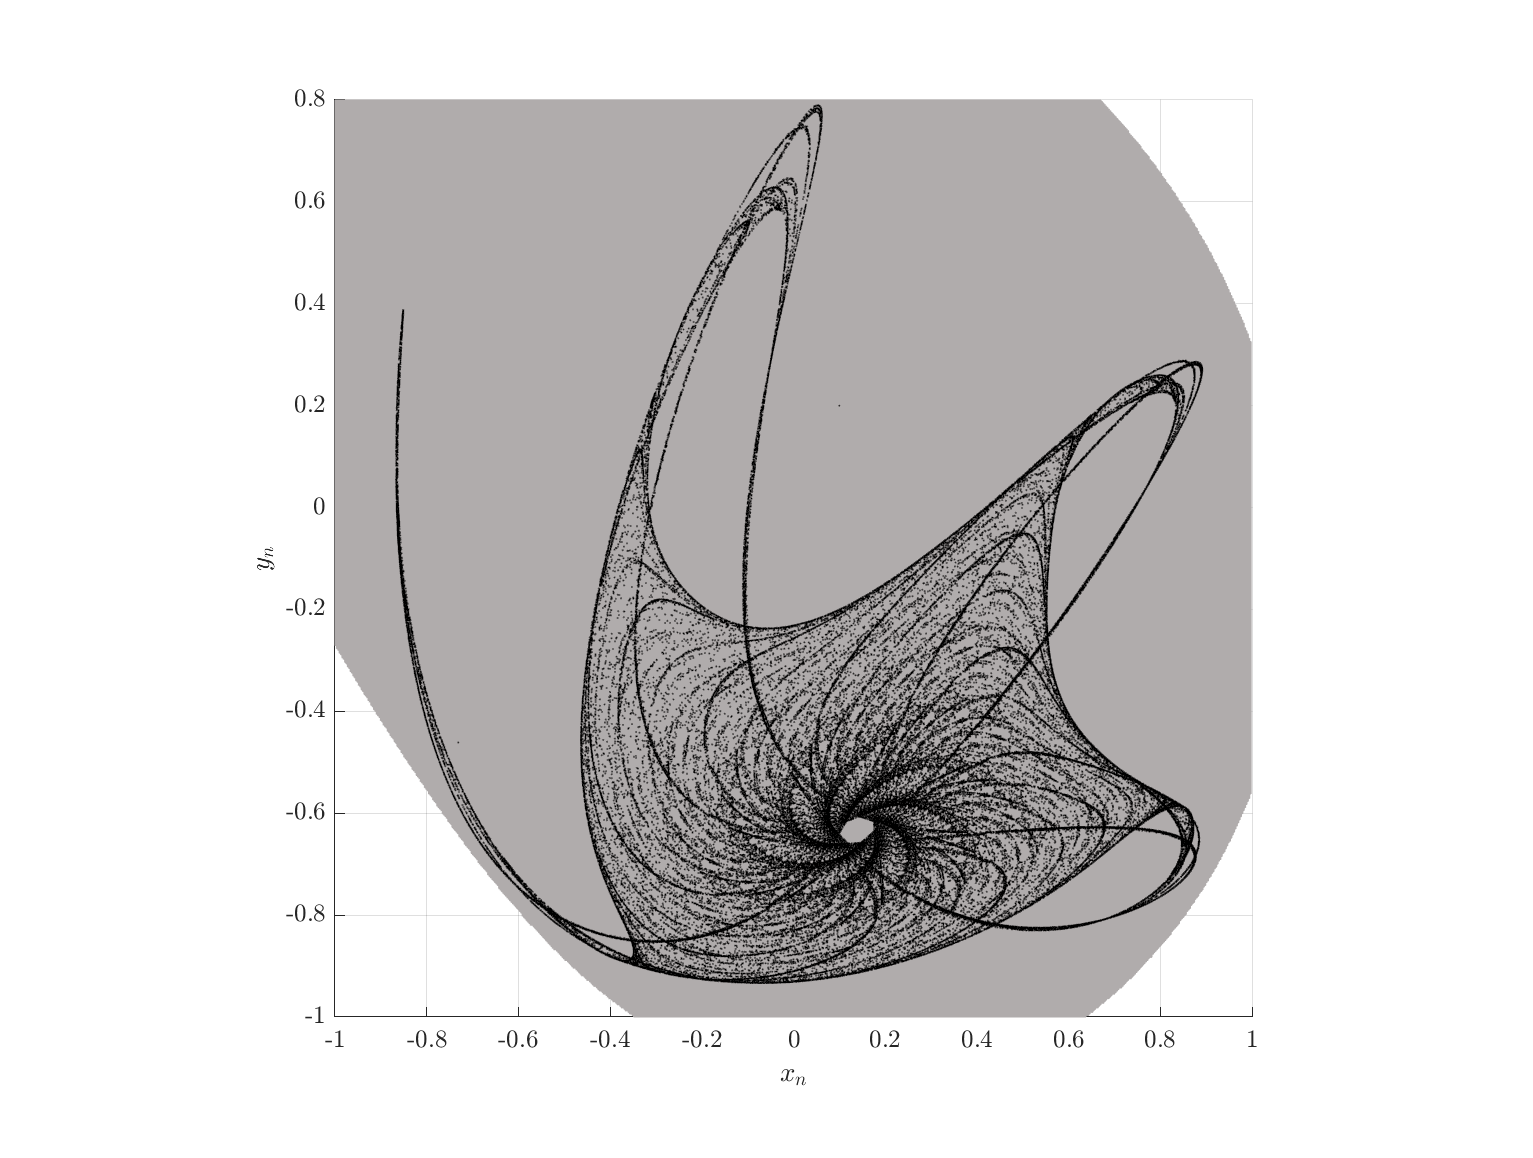
\includegraphics[width=\textwidth,trim=70 0 70 0,clip]{H1_map1}
                \caption{Atractor 1.}    
                \label{fig:mapa_h1}
            \end{subfigure}
            \hfill
            \begin{subfigure}[b]{0.475\textwidth}  
                \centering 
                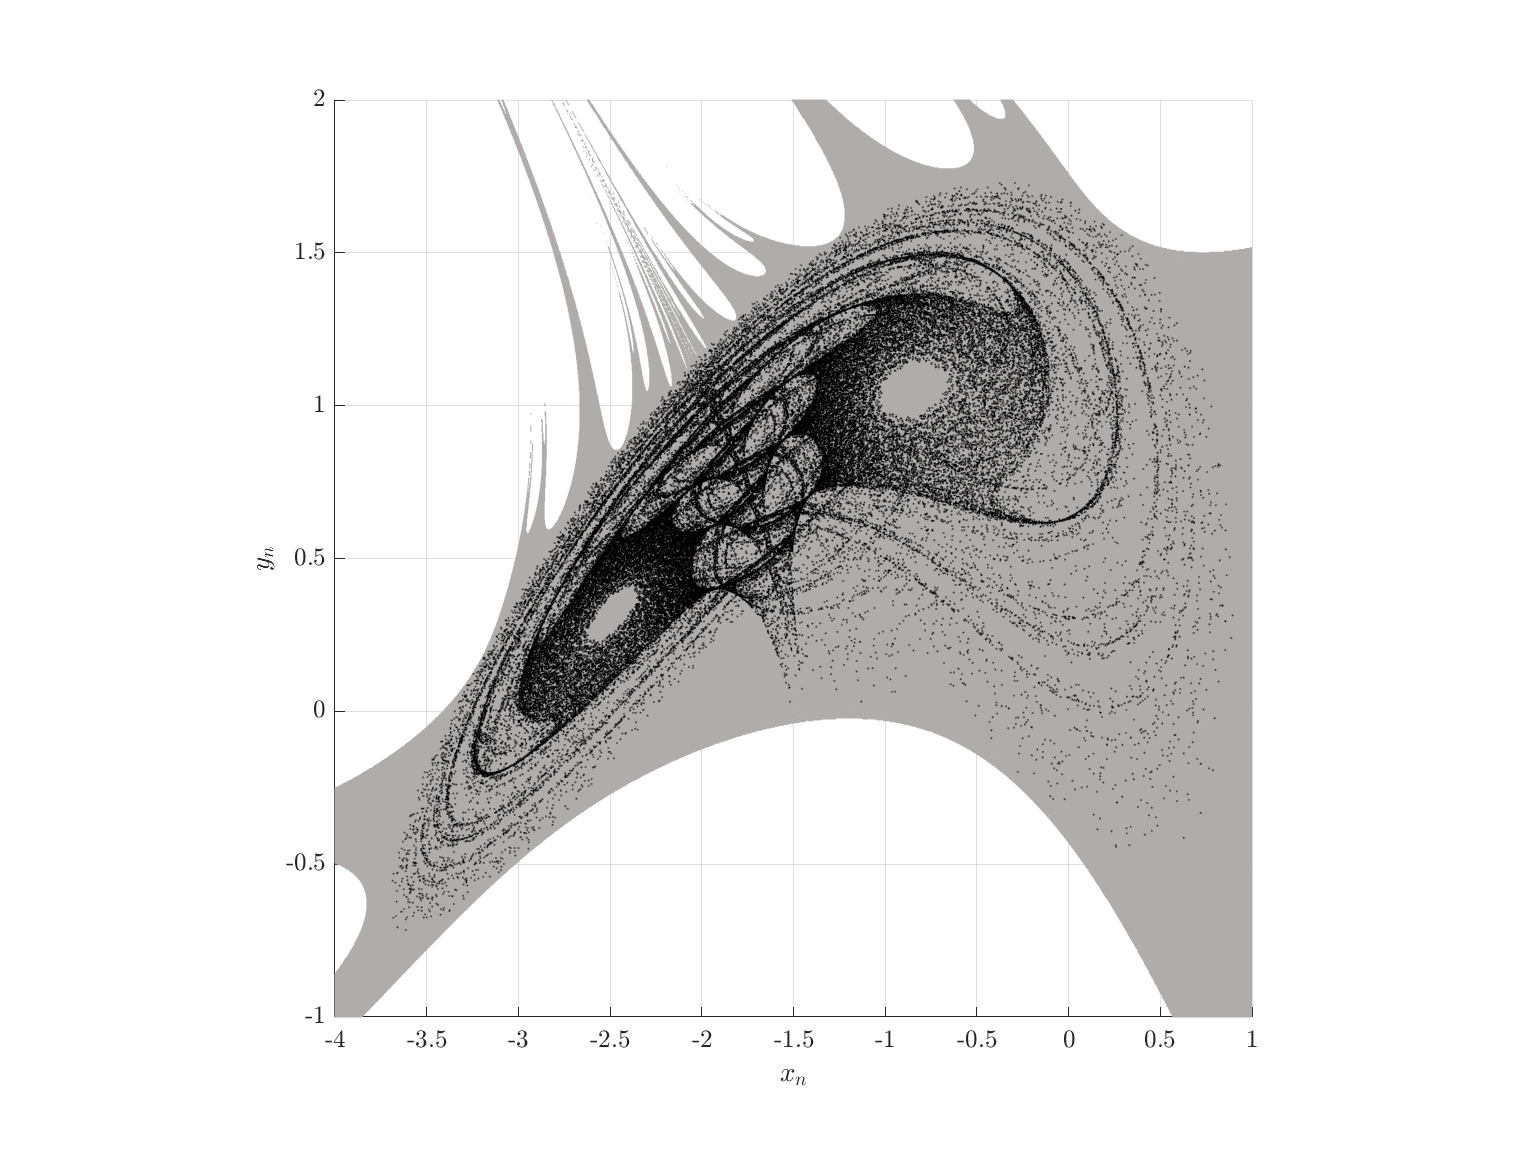
\includegraphics[width=\textwidth,trim=70 0 70 0,clip]{H2_map2}
                \caption{Atractor 2.}    
                \label{fig:mapa_h2}
            \end{subfigure}
        \end{figure}
\end{frame}


% Slide
\begin{frame}
    \frametitle{Mapa caótico}
	\begin{figure}[hbtp]
            \centering
            \caption{Diferentes atractores caóticos y dominios de atracción del mapa bidimensional $A_{3}$ y $A_{4}$.} 
            \begin{subfigure}[b]{0.475\textwidth}   
                \centering 
                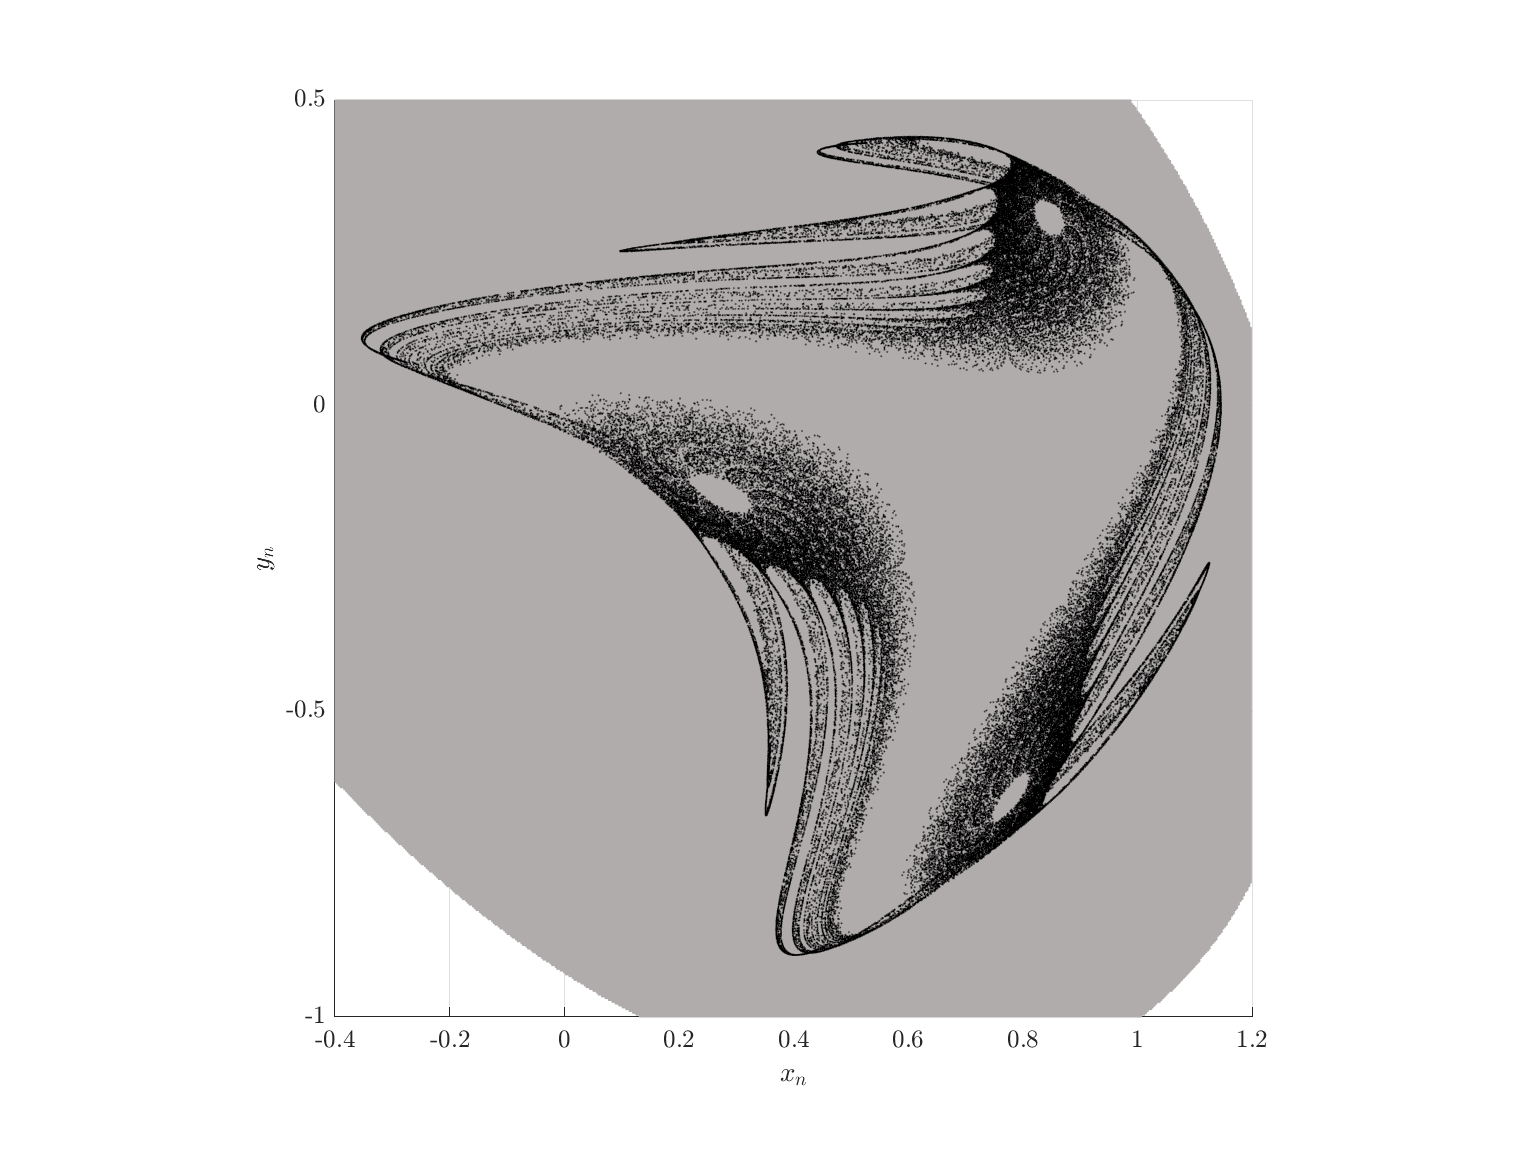
\includegraphics[width=\textwidth,trim=70 0 70 0,clip]{H3_map3}
                \caption{Atractor 3.}    
                \label{fig:mapa_h3}
            \end{subfigure}
            \hfill
            \begin{subfigure}[b]{0.475\textwidth}   
                \centering 
                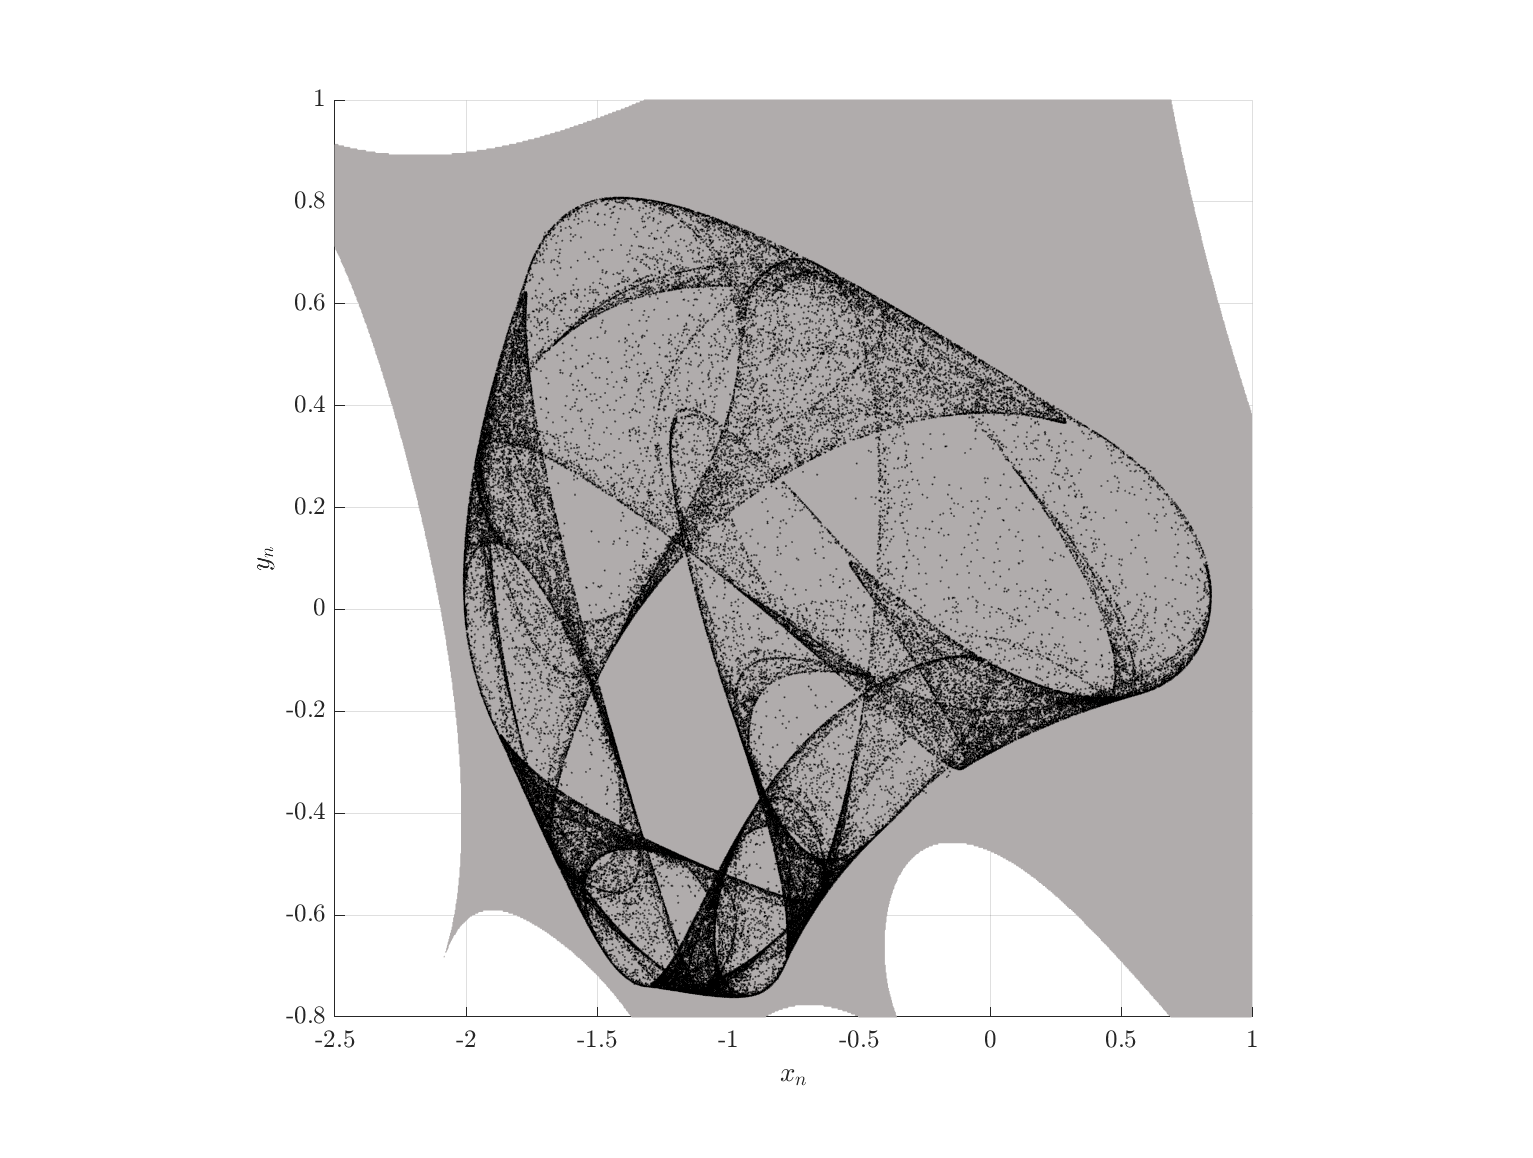
\includegraphics[width=\textwidth,trim=70 0 70 0,clip]{H4_map4}
                \caption{Atractor 4.}    
                \label{fig:mapa_h4}
            \end{subfigure}
        \end{figure}
\end{frame}



% Slide
\begin{frame}
    \frametitle{Mapa caótico}
    \begin{block}{Rangos de condición inicial seleccionados seleccionados}
        \justifying
        \begin{table}[htbp]
            \centering
            \caption{Rangos usados para la condición inicial para cada uno de los atractores.}
            \begin{tabular}{|l|l|}
                \hline
                \rowcolor{lightgray} Atractor  & Rango de valores para $x_{0}$ y $y_{0}$ \\
                \hline
                $1$  & $x_{0} \in [-0.5, \phantom{-} 0.5]$, $y_{0} \in [-0.5, \phantom{-}0.5]$ \\
                \hline
                $2$  & $x_{0} \in [-1.0, \phantom{-} 0.0]$, $y_{0} \in [\phantom{-}0.0, \phantom{-}1.0]$ \\
                \hline
                $3$  & $x_{0} \in [\phantom{-}0.0, \phantom{-} 1.0]$, $y_{0} \in [-0.6, \phantom{-}0.4]$ \\
                \hline
                $4$  & $x_{0} \in [-1.5, -0.5]$, $y_{0} \in [-0.5, \phantom{-}0.5]$ \\
                \hline
            \end{tabular}
            \label{tab:rangos_mapas}
        \end{table} 
        \end{block}
\end{frame}


% Slide
\begin{frame}
    \frametitle{Mapa caótico}
    \begin{block}{DRNG utilizando un mapa caótico bidimensional}
        \justifying
        En \cite{Fraga2021} se utiliza el mapa caótico bidimensional para diseñar un generador de números \textbf{pseudoaleatorios} utilizando una arquitectura de punto fijo y extracción de 16 bits aleatorios haciendo uso de la operación mod 256.
        \begin{equation*}
            \begin{array}{ccl}
                x_{n+1} & = &  a_{1} + a_{2}x_{n} + a_{3}x_{n}^{2} + a_{4}x_{n}y_{n} + a_{5}y_{n} + a_{6}y_{n}^{2}\\
                y_{n+1} & = &  a_{7} + a_{8}x_{n} + a_{9}x_{n}^{2} + a_{10}x_{n}y_{n} + a_{11}y_{n} + a_{12}y_{n}^{2}
            \end{array}
	    \end{equation*}
	    
	    \begin{equation}
            \begin{array}{lcl}
                s_{n+1} = \{ x_{n+1} \text{ mod } 256, y_{n+1} \text{ mod } 256 \}
            \end{array}
            \label{eq:extraccion}
        \end{equation}
	\end{block}
\end{frame}


% Slide
\begin{frame}
    \frametitle{Mapa caótico}
    \begin{block}{Generadores de números aleatorios deterministas (DRNG/PRNG) }
        \justifying
        También conocidos pseudoaleatorios,
        \begin{itemize}
            \item Tienen una forma matemática definida (algoritmo).
            \item Fáciles de implementar en dispositivos lógicos.
            \item Utilizan valores de inicialización llamados semillas.
            \item Para cada semilla se genera una secuencia diferente.
            \item Tienen buenas propiedades estadísticas.
            \item Altas tasas de bits de salida.
        \end{itemize}
	\end{block}
\end{frame}


% Slide
\begin{frame}
    \frametitle{Mapa caótico}
    \begin{block}{Representaciones de números decimales en dispositivos digitales}
        \justifying
         \begin{itemize}
             \item Punto flotante
                 \begin{itemize}
                     \item Mayor rango dinámico.
                     \item Útil en algoritmos complejos.
                 \end{itemize}
             \item Punto fijo
             \begin{itemize}
                     \item Más rápida.
                     \item Menos recursos.
                     \item $X(a,b)$, $a$ bits enteros, $b$ bits fraccionarios, 1 bit de signo.
                     \item Rango $[-2^{a}, 2^{a} - 2^{-b}]$.
                     \item Precisión $2^{-b}$.
                 \end{itemize}
         \end{itemize}
         
         Es preferible utilizar punto fijo en FPGAs.
	\end{block}
\end{frame}


% Slide
\begin{frame}
    \frametitle{Mapa caótico}
    \begin{block}{Análisis de punto fijo}
        \justifying
        Una vez definido el sistema y los atractores a utilizar hay que seleccionar el formato de punto fijo óptimo para cada atractor. Como ejemplo utilizaremos el Atractor 1. 
        \begin{itemize}
            \item Esta acotado en un rango de $x_{n} \in [-0.866, 0.8915]$ y $y_{n} \in [-0.933, 0.7896]$.
            \item Las operaciones que pueden generar los números con magnitud más grandes son la combinación de algunas de las sumas.
            \item Como $|a_{n}| < 1$, con la excepción de $a_{3}$, después de realizar la multiplicación por cualquiera de ellos el número se vuelve más pequeño.
            \item Las combinaciones de sumas que puedan generar el número más grande ($\beta$), donde $a$ son los bits para parte entera:
            \begin{equation}
                a = \log_{2} ( \text{abs}( \beta ) )
                \label{eq:bits_enteros}
            \end{equation}
        \end{itemize}
    
	\end{block}
\end{frame}


% Slide
\begin{frame}
    \frametitle{Mapa caótico}
    \begin{block}{Simulador de punto fijo en C}
        \justifying
         Diseño un simulador de punto fijo en lenguaje C para poder comprobar la factibilidad de la arquitectura antes de pasar al diseño en hardware en FPGA. ¿Cuántos bits de precisión se necesitan?.
        
        \begin{table}[htbp]
            \centering
            \caption{Número de bits usados en la implementación de cada uno de los atractores con aritmética de punto fijo.}
            \resizebox{0.9\linewidth}{!}{
            \begin{tabular}{|l|l|l|l|l|}
                \hline
                \rowcolor{lightgray} Atractor  & Bits parte entera & Bits parte fraccionaria & Rango  & Precisión\\
                \hline
                1     & 3                   & 60   & $[-8.0, 8.0]$   & $8.6739 \times 10^{-19}$\\
                \hline
                2     & 4                   & 59   & $[-16.0, 16.0]$ & $1.7347 \times 10^{-18}$\\
                \hline
                3     & 4                   & 59   & $[-16.0, 16.0]$ & $1.7347 \times 10^{-18}$\\
                \hline
                4     & 3                   & 60   & $[-8.0, 8.0]$   & $8.6739 \times 10^{-19}$\\
                \hline
            \end{tabular}
            }
            \label{tab:bits_atractores}
        \end{table}

	\end{block}
\end{frame}


% Slide
\begin{frame}
    \frametitle{Mapa caótico}
	\begin{figure}[hbtp]
            \centering
            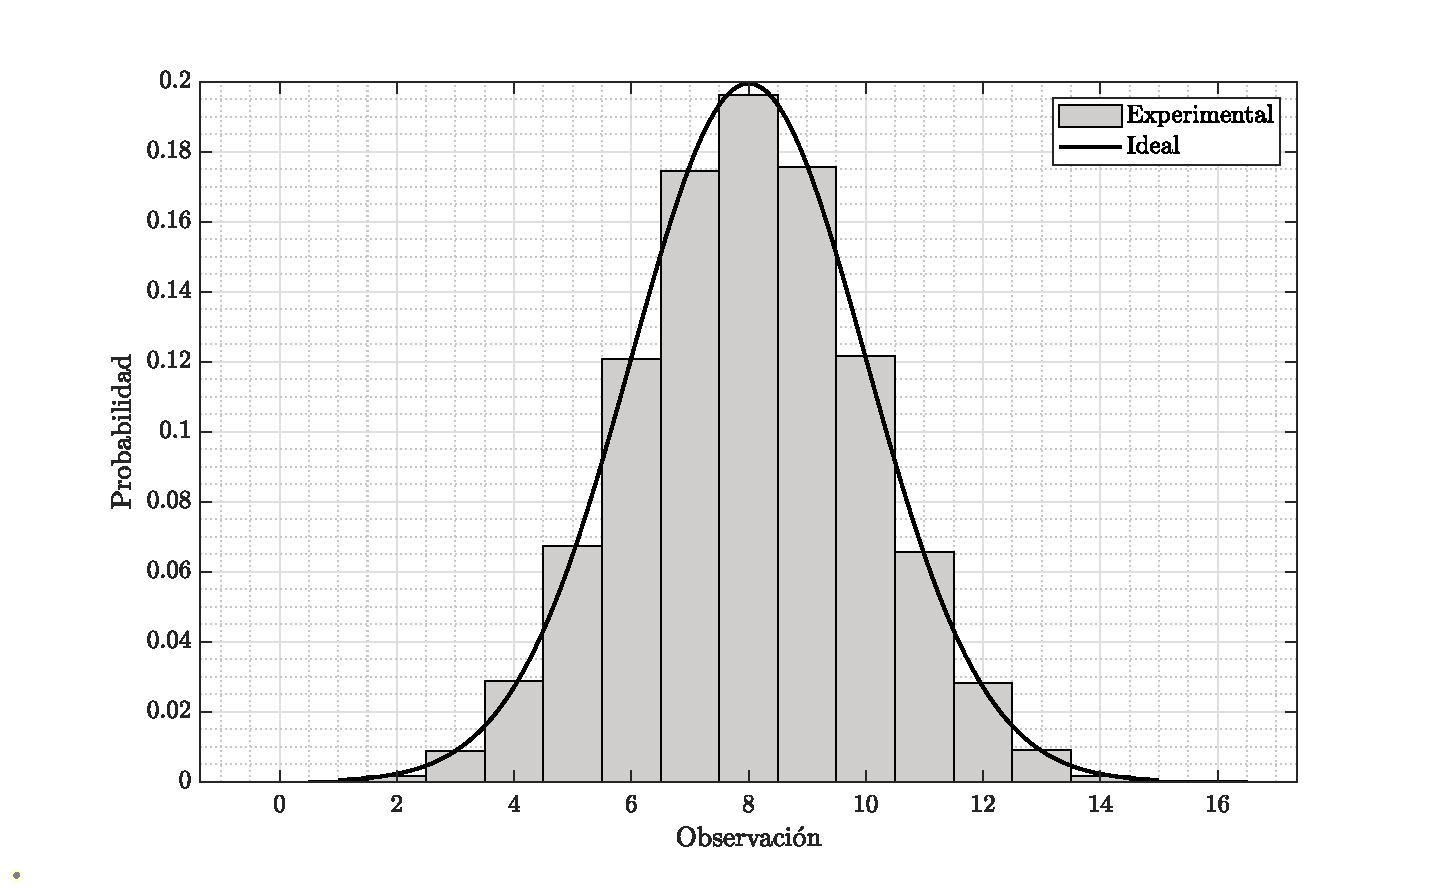
\includegraphics[width=0.8\linewidth]{J0_distribucion_exp}
            \caption{Distribución de 100 millones de palabras de 16 bits.}
            \label{fig:J0_distribucion_exp}
        \end{figure}
\end{frame}

% Slide
\begin{frame}
    \frametitle{Mapa caótico}
    \begin{block}{Implementación en FPGA}
        \justifying
        Si reescribimos la ecuación (\ref{eq:mapa_caotico})  se pueden eliminar dos multiplicadores más. Es decir la mínima cantidad de operaciones que se requieren para implementar el mapa son 10 sumadores y 11 multiplicadores.
        \begin{equation}
            \begin{array}{ccl}
                     x_{n+1} & = &  a_{1} + ( a_{2} + a_{3}x_{n} )x_{n} + a_{4}x_{n}y_{n} + ( a_{5} + a_{6}y_{n} )y_{n} \\
                    y_{n+1} & = &  a_{7} + ( a_{8} + a_{9}x_{n} )x_{n} + a_{10}x_{n}y_{n} + ( a_{11} + a_{12}y_{n})y_{n}
                \end{array}
	    \end{equation}
	\end{block}
\end{frame}


% Slide
\begin{frame}
    \frametitle{Mapa caótico}
        \begin{figure}[hbtp]
            \centering
            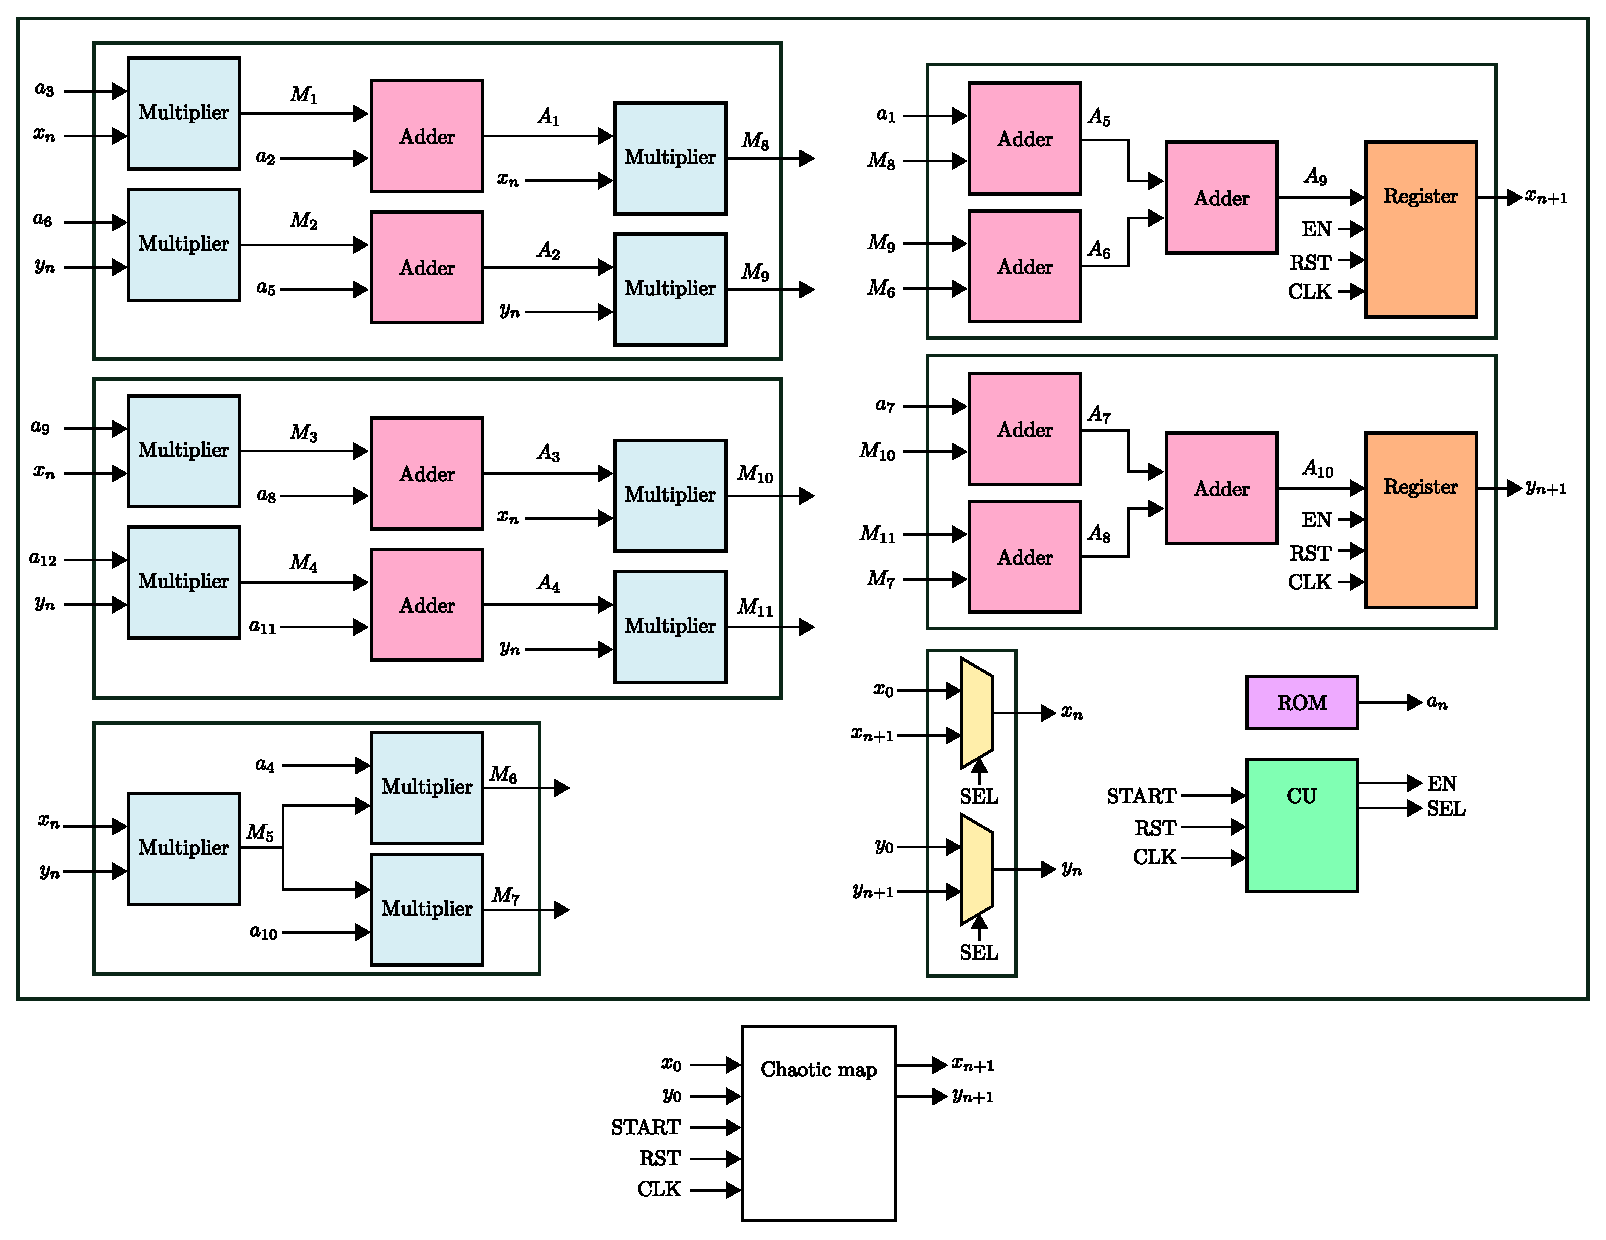
\includegraphics[width=0.8\linewidth]{B1_architecture}
            \caption{Diagrama de bloques del mapa caótico.}
            \label{fig:B1_architecture}
        \end{figure}
\end{frame}

% Slide
\begin{frame}
    \frametitle{Mapa caótico}
        \begin{block}{Máquina de estados de mapa caótico}
            \justifying
            \begin{itemize}
                \item Controlar los multiplexores para seleccionar la condición inicial (SEL).
                \item Controlar los registros de salida que almacenan la iteración actual (EN).
                \item La señal START activa el sistema.
            \end{itemize}
	    \end{block}
        \begin{figure}[hbtp]
            \centering
            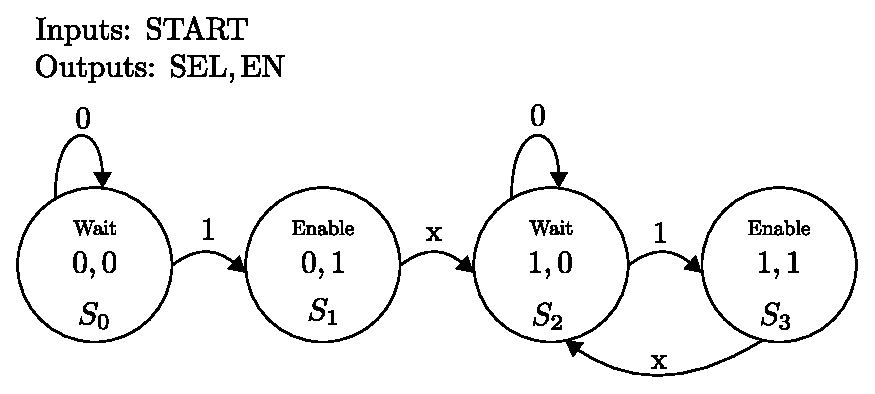
\includegraphics[width=0.6\linewidth]{B2_fsm_cm}
            \caption{Máquina de estados de mapa caótico.}
            \label{fig:B2_fsm_cm}
        \end{figure}
\end{frame}

        
% Slide
\begin{frame}
    \frametitle{Mapa caótico}
        \begin{block}{Multiplicadores de una sola constante (SCM)}
            \justifying
            Al multiplicar por una constante conocida, podemos explotar las propiedades de la multiplicación binaria para obtener un circuito de hardware funcionalmente equivalente con menos recursos lógicos en comparación con un multiplicador genérico. La multiplicación constante puede implementarse como un conjunto de sumas, restas y desplazamientos binarios.
	    \end{block}
	    \begin{figure}[hbtp]
            \centering
            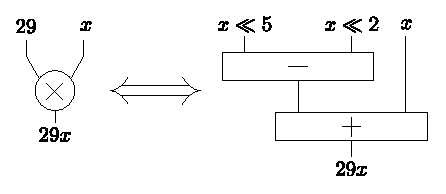
\includegraphics[width=0.6\linewidth]{J1_scm}
            \caption{Ejemplo de multiplicación de una sola constante.}
            \label{fig:J1_scm}
        \end{figure}

\end{frame}

\section{Generador de semillas}

% Slide
\begin{frame}
    \frametitle{Generador de semillas}
    \begin{block}{Descripción de generador de semillas}
        \justifying
        Utiliza un registro de corrimiento a la derecha (RSR) que muestrea el ERO-TNG y compara si 64 bits son extraídos y si se encuentran dentro del rango del dominio de atracción del mapa caótico utilizando los parámetros del Atractor 1. Un contador de 5 bits de una sola vuelta asegura que se hayan generado 64 bits y no pasé una semilla incompleta.
	\end{block}
        \begin{figure}[hbtp]
            \centering
            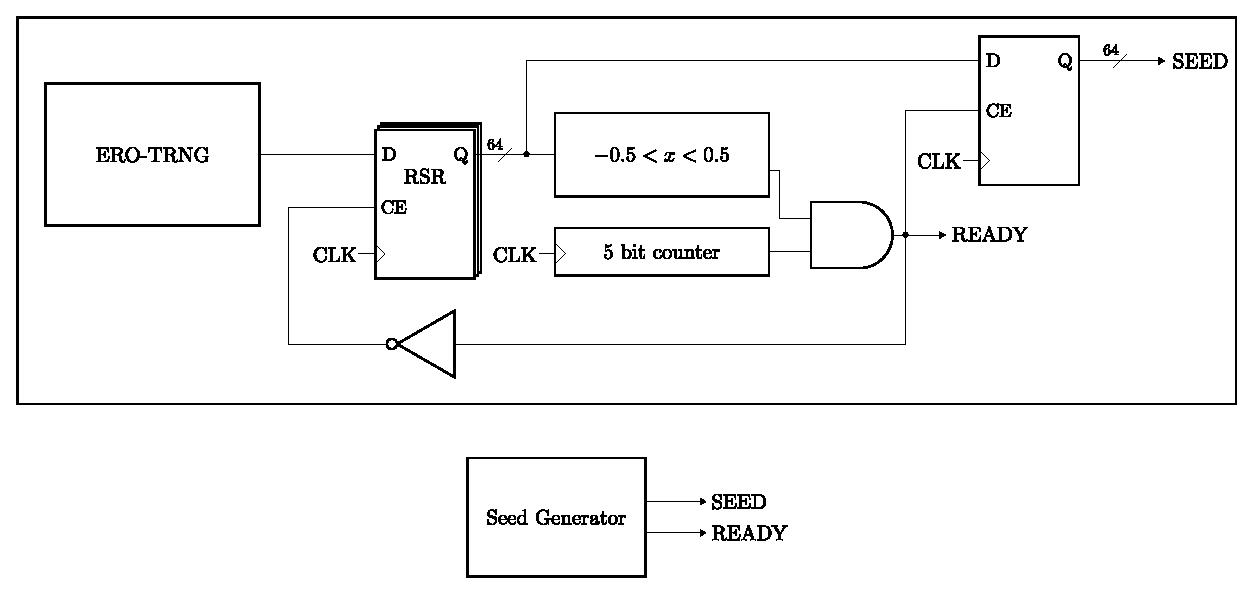
\includegraphics[width=0.8\linewidth]{J2_trng}
            \caption{Generador de semilla.}
            \label{fig:J2_trng}
        \end{figure}
\end{frame}

\section{Implementación de TRNG híbrido}

% Slide
\begin{frame}
    \frametitle{Implementación de TRNG híbrido}
        \begin{figure}[hbtp]
            \centering
            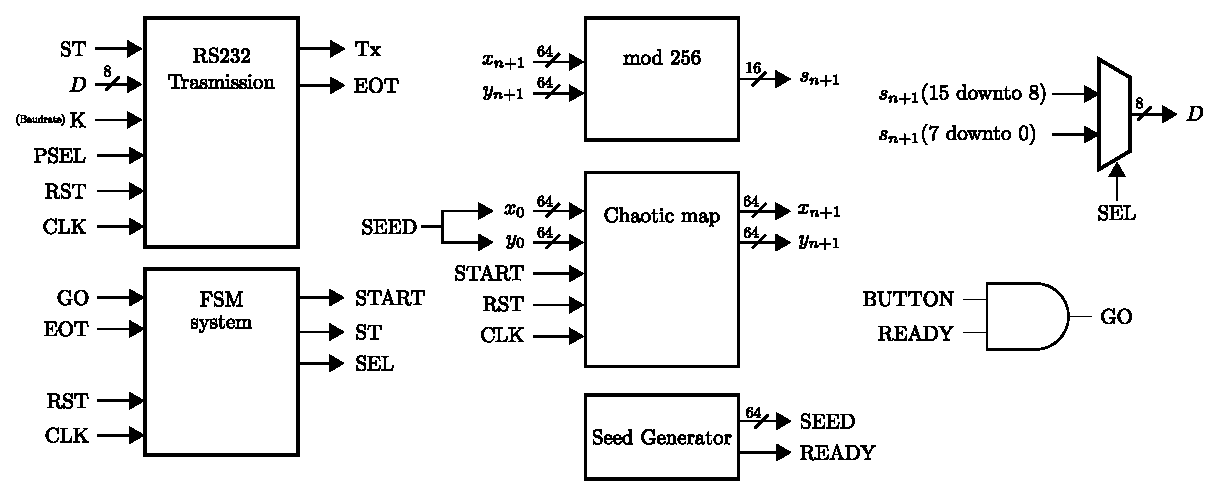
\includegraphics[width=0.99\linewidth]{D0_system}
            \caption{Diagrama de bloques de TRNG híbrido.}
            \label{fig:D0_system}
        \end{figure}
\end{frame}

% Slide
\begin{frame}
    \frametitle{Implementación de TRNG híbrido}
    \begin{block}{Máquina de estados de TRNG híbrido}
        \justifying
        \begin{itemize}
            \item La señal GO activa la máquina de estados del TRNG híbrido.
            \item Calcula una iteración del mapa caótico (START).
            \item Transmite por RS232 los 16 bits aleatorios en dos paquetes de 8 bits.
        \end{itemize}
	\end{block}
        \begin{figure}[hbtp]
            \centering
            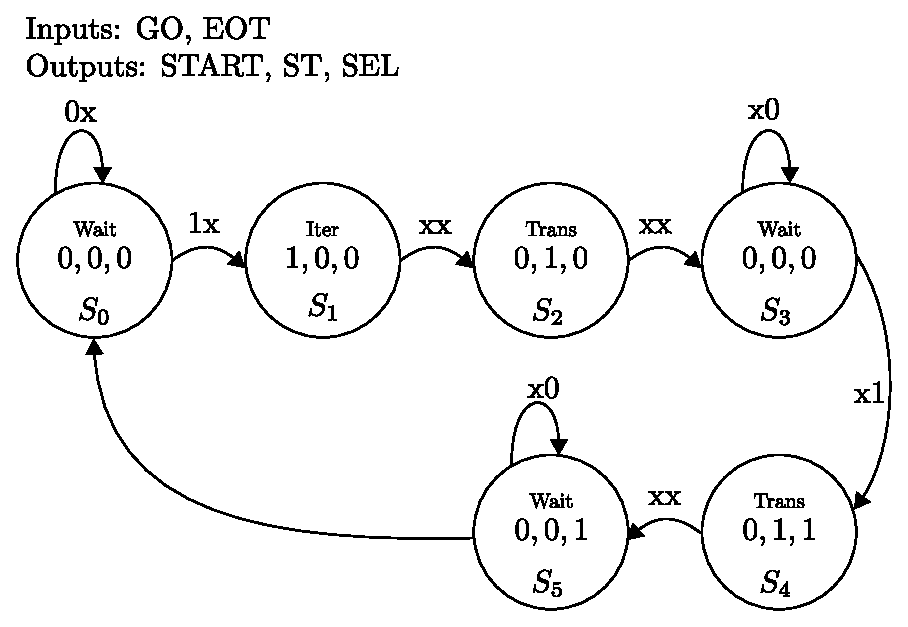
\includegraphics[width=0.5\linewidth]{D1_fsm_system}
            \caption{Máquina de estados de TRNG híbrido.}
            \label{fig:D1_fsm_system}
        \end{figure}
\end{frame}

% Slide
\begin{frame}
    \frametitle{Implementación de TRNG híbrido}
	\begin{figure}[hbtp]
            \centering
            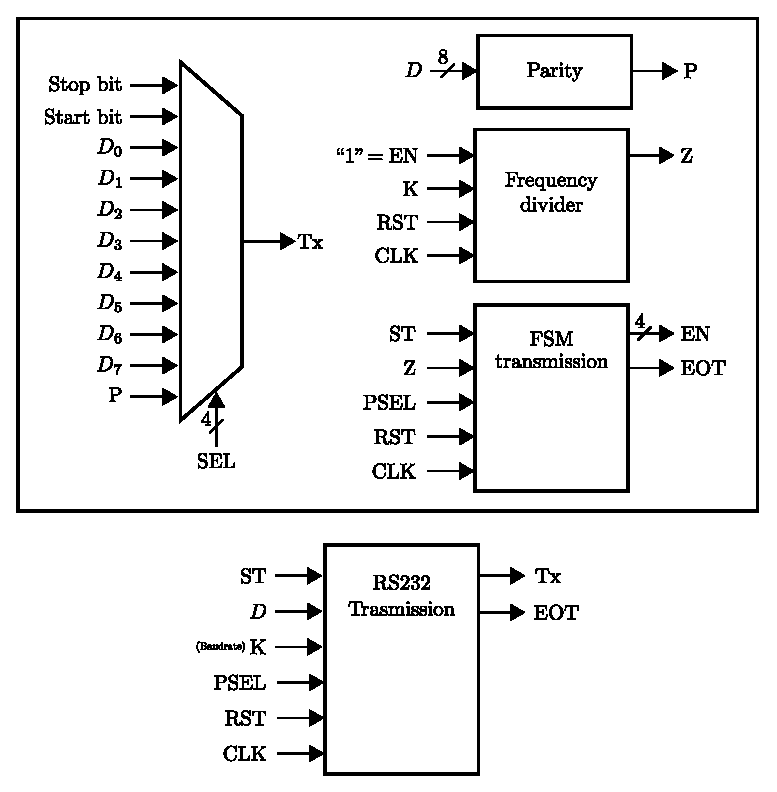
\includegraphics[width=0.5\linewidth]{C1_architecture_rs232}
            \caption{Diagrama de bloques de transmisión RS232.}
            \label{fig:C1_architecture_rs232}
        \end{figure}
\end{frame}

% Slide
\begin{frame}
    \frametitle{Implementación de TRNG híbrido}
	\begin{figure}[hbtp]
            \centering
            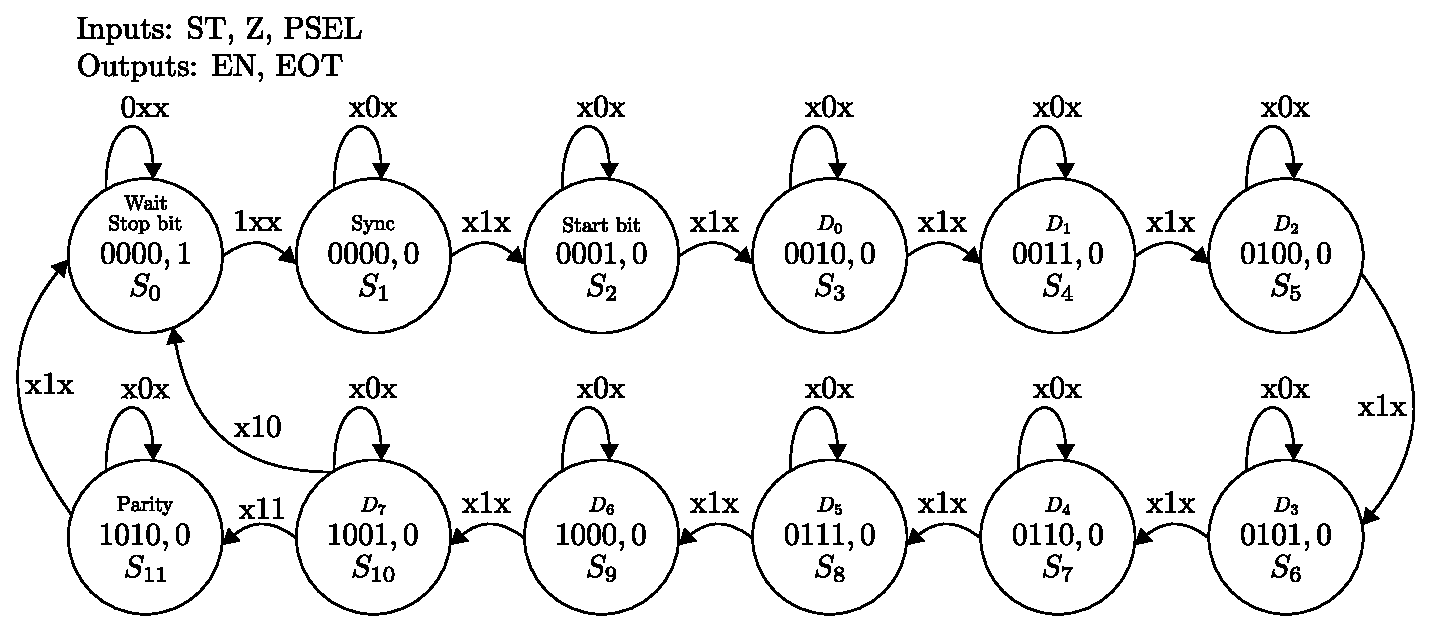
\includegraphics[width=0.8\linewidth]{C0_fsm_rs232}
            \caption{Máquina de estados para la transmisión RS232.}
            \label{fig:C0_fsm_rs232}
        \end{figure}
\end{frame}



\section{Resultados}

% Slide
\begin{frame}
    \frametitle{Resultados}
    \begin{table}[htbp]
    \centering
    \caption{Resultados de la aplicación de las pruebas NIST al TRNG híbrido implementado en aritmética de punto fijo con 100 secuencias de un millón de datos.}
    \resizebox{0.45\linewidth}{!}{
    \begin{NiceTabular}{|l|c|c|}
    \CodeBefore
    \rowcolor{lightgray}{1}
    \Body
    \hline
     Test name                 & p-value  & \%   \\
    \hline
    Frequency                 & 0.383827 & 0.99 \\
    \hline
    Block frequency           & 0.108791 & 1.00 \\
    \hline
    Cumulative sums           & 0.401199 & 1.00 \\
    \hline
    Runs                      & 0.971699 & 0.99 \\
    \hline
    Longest Run               & 0.759756 & 1.00 \\
    \hline
    Rank                      & 0.383827 & 0.99 \\
    \hline
    FFT                       & 0.383827 & 0.99 \\
    \hline
    NonOverlapping template   & 0.480298 & 0.99 \\
    \hline
    Overlapping template      & 0.883171 & 0.99 \\
    \hline
    Universal                 & 0.574903 & 0.99 \\
    \hline
    Approximate entropy       & 0.759756 & 0.98 \\
    \hline
    Random excursions         & 0.265539 & 0.99 \\
    \hline
    Random excursions variant & 0.312463 & 0.99 \\
    \hline
    Serial                    & 0.595604 & 1.00 \\
    \hline
    Linear complexity         & 0.574903 & 1.00 \\
    \hline
    \end{NiceTabular}%
    }
  \label{tab:resultados_NIST_100}%
  \end{table}%
\end{frame}

% Slide
\begin{frame}
    \frametitle{Resultados}
    \begin{table}[htbp]
    \centering
    \caption{Resultados de la aplicación de las pruebas NIST al TRNG híbrido implementado en aritmética de punto fijo con 1000 secuencias de un millón de datos.}
    \resizebox{0.45\linewidth}{!}{
    \begin{NiceTabular}{|l|c|c|}
    \CodeBefore
    \rowcolor{lightgray}{1}
    \Body
    \hline
    Test name                 & p-value  & \%   \\
    \hline
    Frequency                 & 0.587274 & 0.989 \\
    \hline
    Block frequency           & 0.796268 & 0.998 \\
    \hline
    Cumulative sums           & 0.848047 & 0.990 \\
    \hline
    Runs                      & 0.614226 & 0.988 \\
    \hline
    Longest Run               & 0.660012 & 0.992 \\
    \hline
    Rank                      & 0.255705 & 0.990 \\
    \hline
    FFT                       & 0.072514 & 0.994 \\
    \hline
    NonOverlapping template   & 0.481082 & 0.989 \\
    \hline
    Overlapping template      & 0.143686 & 0.988 \\
    \hline
    Universal                 & 0.228367 & 0.988 \\
    \hline
    Approximate entropy       & 0.786830 & 0.992 \\
    \hline
    Random excursions         & 0.447308 & 0.990 \\
    \hline
    Random excursions variant & 0.405096 & 0.992 \\
    \hline
    Serial                    & 0.124135 & 0.993  \\
    \hline
    Linear complexity         & 0.008816 & 0.989 \\
    \hline
    \end{NiceTabular}%
    }
  \label{tab:resultados_NIST_1000}%
   \end{table}%
\end{frame}

% Slide
\begin{frame}
    \frametitle{Resultados}
    \begin{figure}[hbtp]
            \centering
            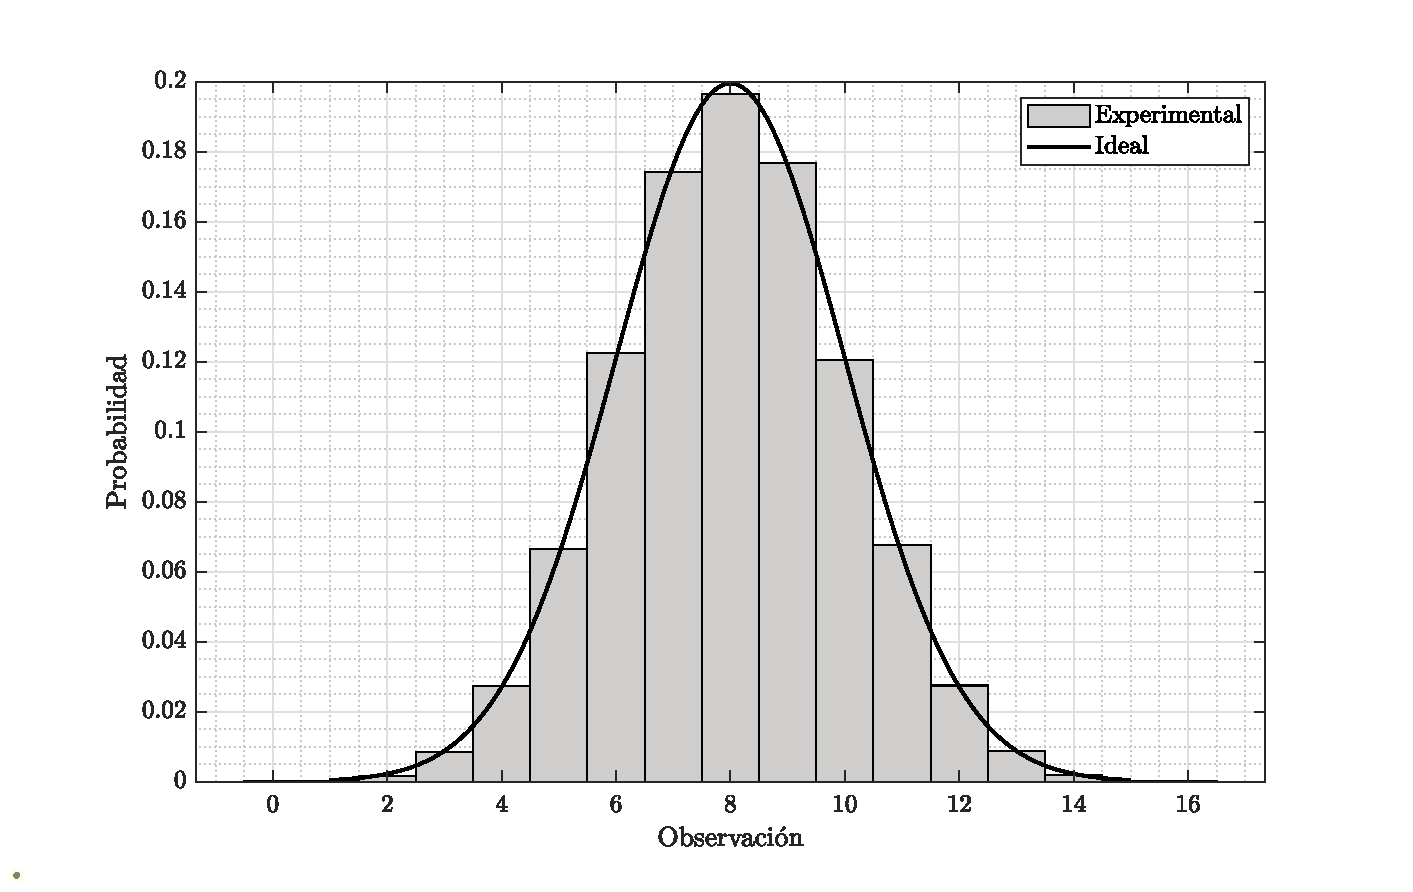
\includegraphics[width=0.8\linewidth]{J3_distribucion}
            \caption{Distribución de 100 millones de palabras de 16 bits experimentales.}
            \label{fig:J3_distribucion}
        \end{figure}
\end{frame}

% Slide
\begin{frame}
    \frametitle{Resultados}
         \begin{figure}[hbtp]
            \centering
            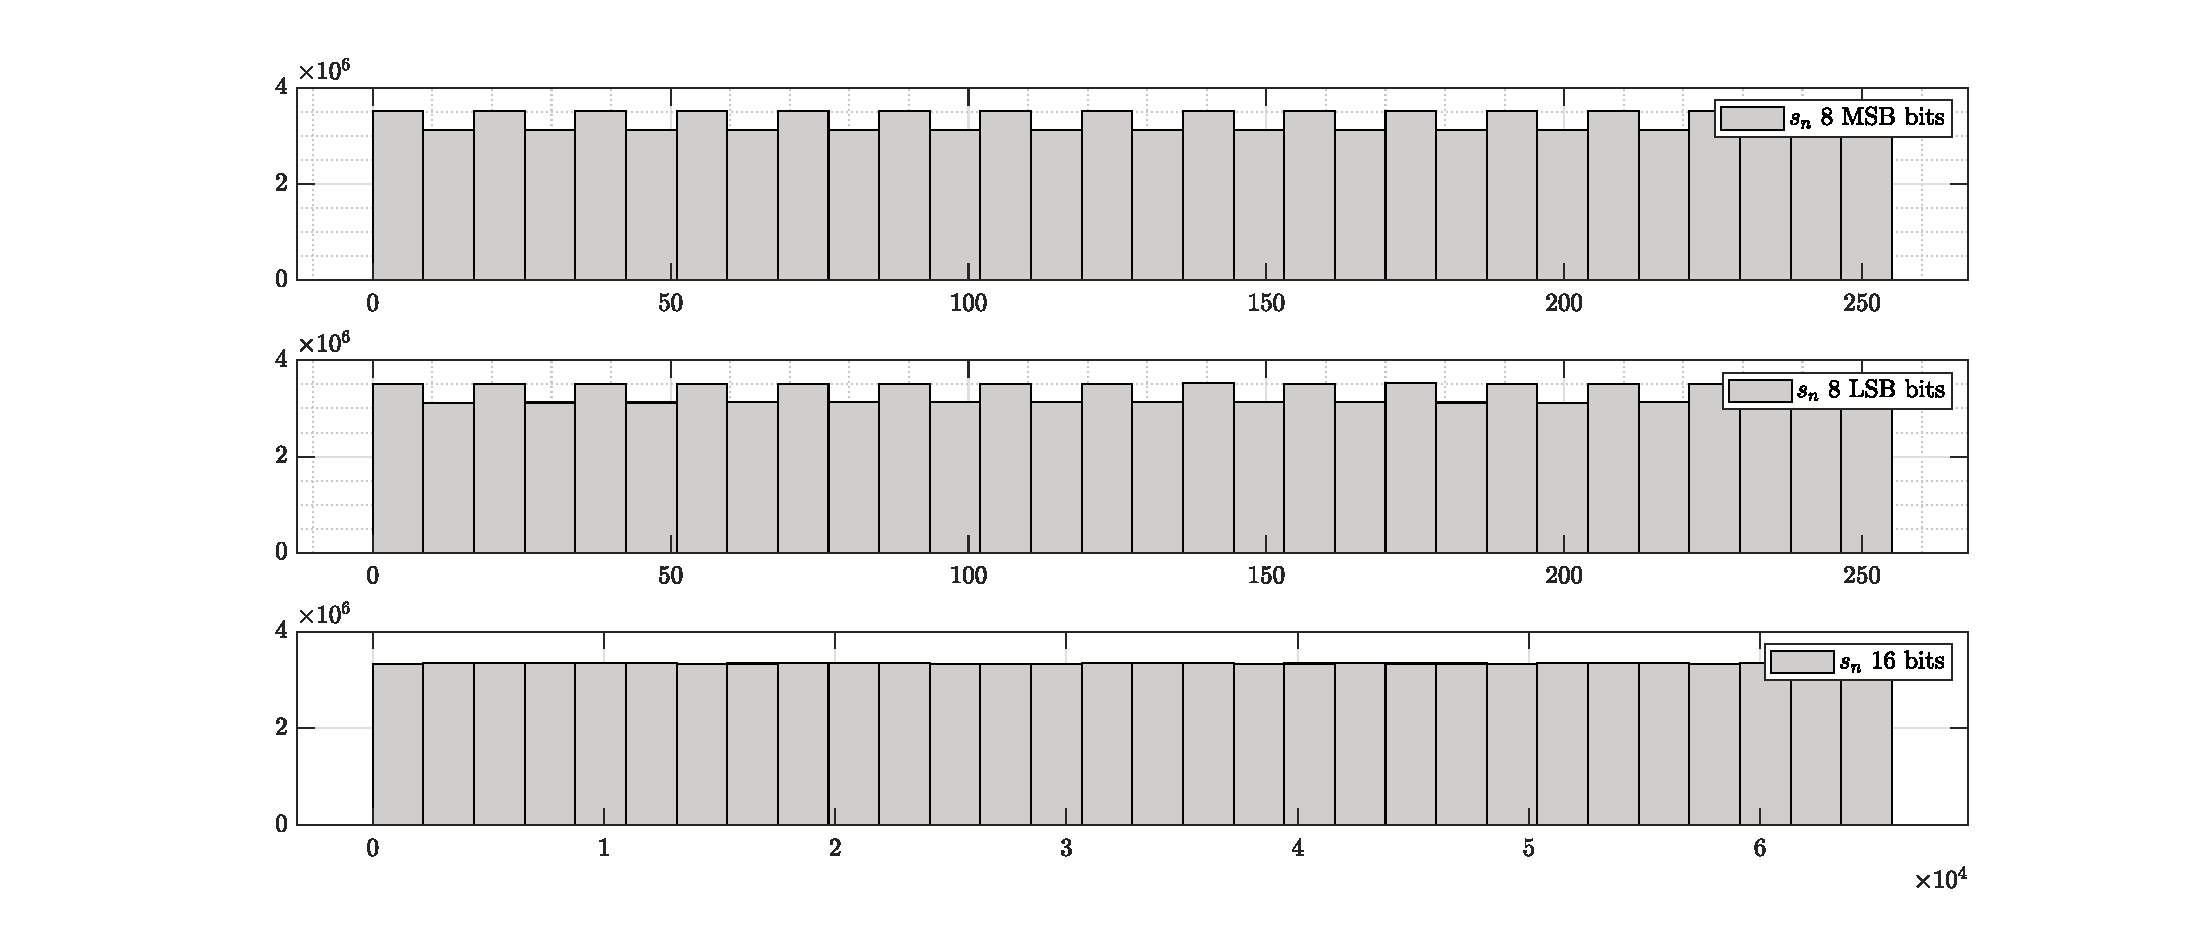
\includegraphics[width=0.95\linewidth]{Z4_distribucion_normal}
            \caption{Histograma de resultados experimentales primeros 100 mil secuencias binarias.}
            \label{fig:J4_distribucion}
        \end{figure}
\end{frame}


% Slide
\begin{frame}
    \frametitle{Resultados}
	 \begin{table}[htbp]
            \centering
            \caption{Uso de recursos del TRNG híbrido con multiplicadores completos.}
            \resizebox{0.45\linewidth}{!}{
            \begin{tabular}{|l|l|l|l|}
                \hline
                \rowcolor{lightgray} Recursos  & Utilización & Disponibles & Utilización \% \\
                \hline
                LUTs      & 17767  & 20800    & 85.42  \\
                \hline
                FF     &  148 & 41600   & 0.36 \\
                \hline
                DSP       & 90  & 90   & 100.0 \\
                \hline
            \end{tabular}
            }
            \label{tab:recursos}
        \end{table}

        \begin{table}[htbp]
            \centering
            \caption{Uso de recursos del TRNG híbrido con multiplicadores de una sola constante en parámetros $a_{n}$.}
            \resizebox{0.45\linewidth}{!}{
            \begin{tabular}{|l|l|l|l|}
                \hline
                \rowcolor{lightgray} Recursos  & Utilización & Disponibles & Utilización \% \\
                \hline
                LUTs      & 1469  & 20800    & 7.06  \\
                \hline
                FF     & 146  & 41600   & 0.35  \\
                \hline
                DSP       & 80  & 90   & 88.89  \\
                \hline
            \end{tabular}
            }
            \label{tab:recursos_op}
        \end{table}
        
        \begin{block}{}
            \justifying
            La velocidad obtenida por el TRNG híbrido fue de 533.33 Mbit/s, es ligeramente superior a sistemas similares las cuales rondan los 400 Mbit/s.
        \end{block}
         
\end{frame}


\section{Conclusión}

% Slide
\begin{frame}
    \frametitle{Publicaciones}
    \begin{block}{Publicaciones generadas durante la maestría}
        \justifying
        \begin{scriptsize}
            \begin{enumerate} 
            \item[(1)] C. García-Grimaldo, C. F. Bermudez-Marquez, E. Tlelo-Cuautle, and E. Campos-Cantón, ``FPGA implementation of a chaotic map with no fixed point,'' Electronics, vol. 12, p. 444, jan 2023.

            \item[(2)] S. Vaidyanathan, A. Sambas, E. Tlelo-Cuautle, C. F. Bermudez-Marquez, K. Benkouider, and S. A. Safaan, ``A new hyperchaotic two-scroll system: Bifurcation study, multistability, circuit simulation, and FPGA realization,'' Discrete Dynamics in Nature and Society, vol. 2022, pp. 1–17, sep 2022.

            \item[(3)] K. Benkouider, S. Vaidyanathan, A. Sambas, E. Tlelo-Cuautle, A. A. A. El-Latif, B. Abd-El-Atty, C. F. Bermudez-Marquez, I. M. Sulaiman, A. M. Awwal, and P. Kumam, ``A new 5-d multistable hyperchaotic system with three positive lyapunov exponents: Bifurcation analysis, circuit design, FPGA realization and image encryption,'' IEEE Access, vol. 10, pp. 90111–90132, 2022.

            \item[(4)] S. Vaidyanathan, I. Moroz, E. Tielo-Cuautle, A. Sambas, C. Bermudez-Marquez, and S. Safaan, ``Mathematical modelling, bifurcation analysis, circuit design and fpga implementation of a 5-d hyperchaotic weather fluctuation model with a line of equilibrium points,'' International Journal of Modelling, Identification and Control, 2022. (En revisión)
            \end{enumerate}

        \end{scriptsize}
        
	\end{block}
\end{frame}


% Slide
\begin{frame}
    \frametitle{Conclusión}
    \begin{block}{Conclusiones}
        \justifying
        \begin{itemize}
        \item El núcleo ERO-TRNG tienen un modelo estocástico bien definido y forma parte de los núcleos aprobados por la AIS20/31.

        \item Se tienen 12 parámetros diferentes para configurarse lo que lo hace muy versátil (diferentes atractores).

        \item La implementación utiliza un 88\% de los DPS y tan solo un 7\% de los LUTs de la FPGA, no obstante considerando que la FPGA utilizada es de bajos recursos, para FPGAs más grandes las cuales tienen de 4 a 5 recursos, este sistema no representa un gran consumo de área.

        \item El TRNG híbrido pasó todas las pruebas NIST y el análisis estadístico demostró distribuciones uniformes.

        \item La velocidad obtenida por el TRNG híbrido fue de 533.33 Mbit/s, es ligeramente superior a sistemas similares las cuales rondan los 400 Mbit/s.

    \end{itemize}

	\end{block}
\end{frame}

% Slide
\begin{frame}
    \frametitle{Conclusión}
    \begin{block}{Conclusiones}
        \justifying
        \begin{itemize}
        \item Se diseño un simulador en C para comprobar arquitecturas de punto fijo.
        \item Es repetible en diferentes familias de FPGAs de Xilinx.
    \end{itemize}

	\end{block}
\end{frame}




\section{Bibliografía}

% Slide
\begin{frame}[t, allowframebreaks]
    \frametitle{Bibliografía}
    %\nocite{*}
	\bibliographystyle{ieeetr}
	\bibliography{../bibliografia}
\end{frame}


\end{document}
